\documentclass[11 pt, reqno]{amsart}
\usepackage{amssymb,amsmath}
\usepackage{hyperref, cite}
\usepackage{epsfig}
\newtheorem{theorem}{Theorem}[section]
\newtheorem{corollary}[theorem]{Corollary}
\newtheorem{lemma}[theorem]{Lemma}
\newtheorem{proposition}[theorem]{Proposition}
\theoremstyle{definition}
\newtheorem{conjecture}[theorem]{Conjecture}
\newtheorem{question}[theorem]{Question}
\newtheorem{problem}[theorem]{Problem}
\newtheorem{definition}[theorem]{Definition}
\newtheorem{example}[theorem]{Example}
\newtheorem{remark}[theorem]{Remark}
\numberwithin{equation}{subsection}
\newtheorem*{ack}{Acknowledgement}
\usepackage[all,cmtip]{xy}
\usepackage{float}
\usepackage{multicol}
\newcommand{\Aut}{\operatorname{Aut}}
\newcommand{\id}{\mathrm{id}}
\newcommand{\overbar}[1]{\mkern 1.5mu\overline{\mkern-1.5mu#1\mkern-1.5mu}\mkern 1.5mu}
\newcommand{\RNum}[1]{\uppercase\expandafter{\romannumeral #1\relax}}
\setlength\oddsidemargin{.8mm}
\setlength\evensidemargin{.8mm}
\setlength\textheight{21cm}
\setlength\textwidth{16cm}
\usepackage[autostyle]{csquotes}
\usepackage{color}

\begin{document}
\title{Virtually symmetric representations and marked Gauss diagrams}


\author{Valeriy G. Bardakov}
\address{Sobolev Institute of Mathematics, 4 Acad. Koptyug avenue, 630090, Novosibirsk, Russia.}
\address{Novosibirsk State  University, 2 Pirogova Street, 630090, Novosibirsk, Russia.}
\address{Novosibirsk State Agrarian University, Dobrolyubova street, 160, Novosibirsk, 630039, Russia.}
\address{Regional Scientific and Educational Mathematical Center of Tomsk State University, 36 Lenin Ave., Tomsk, Russia.}
\email{bardakov@math.nsc.ru}

\author{Mikhail V. Neshchadim}
\address{Sobolev Institute of Mathematics, 4 Acad. Koptyug avenue, 630090, Novosibirsk, Russia.}
\address{Novosibirsk State  University, 2 Pirogova Street, 630090, Novosibirsk, Russia.}
\address{Regional Scientific and Educational Mathematical Center of Tomsk State University, 36 Lenin Ave., Tomsk, Russia}
\email{neshch@math.nsc.ru}

\author{Manpreet Singh}
\address{Department of Mathematical Sciences, Indian Institute of Science Education and Research (IISER) Mohali, Sector 81,  S. A. S. Nagar, P. O. Manauli, Punjab 140306, India.}
\email{manpreetsingh@iisermohali.ac.in}

%\subjclass[2020]{Primary 57K12, 20F36; Secondary 05C10}
\keywords{Virtual knot, Virtual knot group, Virtual spatial graph diagram, Marked Gauss diagram, Marked link diagram, Peripheral subgroup}


\begin{abstract}
In this paper we define virtually symmetric representations of virtual braid group $VB_n$ and prove that many previously known representations are equivalent to virtually symmetric representations. Using a virtually symmetric representation we define virtual link group. We define and study group system of virtual knots by defining marked Gauss diagrams as an extension of Gauss diagrams. A marked Gauss diagram is a Gauss diagram with marked nodes $($signed vertices$)$ on circles, and are not attached to arrows. In particular, we extend the definition of virtual link group to marked Gauss diagrams and define peripheral structure for $1$-circle marked Gauss diagrams. We define $C_m$-groups and prove that every irreducible $C_1$-group can be realized as the group of a marked Gauss diagram. We give an interpretation of marked Gauss diagrams in terms of virtual spatial graph diagrams with marked nodes. We also study peripherally specified homomorphic image of groups associated to marked Gauss diagrams.
\end{abstract}
\maketitle

\section{Introduction}

A link diagram is a generic projection of link onto a plane with over and under crossing information at double points. Two link diagrams are equivalent if they are related by a finite sequence of Reidemeister moves and planar isotopy. To each oriented link diagram one can associate a Gauss diagram and for each Reidemeister move on link diagrams one can describe the corresponding moves on Gauss diagrams. But there are many Gauss diagrams which do not come from link diagrams. In $1996$, L. Kauffman \cite{Kauffman-1} introduced virtual links as a generalization of classical knot theory. A virtual link diagram is a generic immersion of oriented circles into a plane where double points are of two types: either they are decorated with over and under crossing information or they are decorated with a small circle, called virtual crossings. Two virtual link diagrams are said to be equivalent if they are related by a finite sequence of generalized Reidemeister moves. Moreover, there is one-to-one correspondence between equivalence classes virtual link diagrams and equivalence classes of Gauss diagrams. In \cite{GPV-1}, M. Goussarov, M. Polyak and O. Viro studied virtual links in terms of Gauss diagrams and describe finite-type invariants for virtual links. N. Kamada and S. Kamada \cite{KK-1} gave an interpretation of virtual links as link diagrams on oriented surfaces, called abstract link diagrams. Also, G. Kuperberg \cite{Kuperberg-1} studied virtual links as links in thickened surfaces. Analogous to a generalization of classical knot theory to virtual knot theory, there is a generalization of classical braids to virtual braids by L. Kauffman \cite{Kauffman-1}. V. Vershinin \cite{VV-1} gave a presentation of virtual braid group $VB_n$. In \cite{Kamada-1}, S. Kamada proved analogous results of Alexander and Markov theorems for virtual braids. Also, L. H. Kauffman and S. Lambropoulou \cite{KL-1} proved Markov theorem for virtual braids using $L$-moves.
\par 

Unlike the fundamental group of a classical knot, there are several definitions for virtual knot group (see, for example, \cite{Bar-1,BB-1, BB-2, BMN-1, BMN-2, BN-2, BN-3, BDGGHN-1, CSW-1, Kauffman-1, Man, SW-1}). To each virtual link diagram $L$, L. Kauffman \cite{Kauffman-1} assigned a group $G_0(L)$ by a adding generator for each arc from one under crossing to another under crossing and adding relations at classical crossings as done in the case of classical link diagram. One way to associate group to virtual link is via representation of virtual braid group $VB_n$. In this paper we show that many known representations of virtual braid groups $VB_n$ are virtually symmetric, and  have used one such virtually symmetric representation to define virtual link group $G_M(L)$. An advantage of using a virtually symmetric representation is that we can describe virtual link group $G_M(L)$ using Gauss diagrams too. We have also constructed a linear, local, not homogeneous representation of a virtual braid group $VB_n$ and have shown that it is also equivalent to a virtually symmetric representation. 
\par 

In \cite{Kauffman-1}, for each virtual knot $K$ a peripheral subgroup of $G_0(K)$ is also defined. S. Kim \cite{Kim-1} studied this group system and observed many new and unexpected results. This motivates us to define and study group system for virtual knots using groups $G_M(K)$. We define marked Gauss diagrams which generalizes Gauss diagrams, and introduce an equivalence relation on them generated by a sequence of moves, called marked Reidemeister moves. There is a canonical injective map from equivalence classes of Gauss diagrams to equivalence classes of marked Gauss diagrams. A marked Gauss diagram is a Gauss diagram with signed nodes on circles which are not attached to any arrows. For each marked Gauss diagram $D$ we assign a group $\Pi_D$ and define a peripheral subgroup. If $D$ is a Gauss diagram, then the group $\Pi_D$ is isomorphic to the group $G_M(L)$, where $L$ is the virtual link corresponding to $D$. In particular, we can define group system for virtual knots.
\par 

Spatial graph theory $($embedding of a graph in $\mathbb{R}^3)$ is an another extension of classical knot theory. L. Kauffman \cite{Kauffman-2}, S. Yamada \cite{Yamada-1}, and D. Yetter \cite{Yetter-1}, independently introduced Reidemeister moves for spatial graph diagrams. In the paper \cite{FM-1}, T. Fleming and B. Mellor combined the concept of virtual links and spatial graphs and introduced virtual spatial graph theory. In paper \cite{BH-1}, L. Beineke and F. Harary introduced directed graphs in which nodes $($vertices$)$ are assigned either positive or negative sign and called these graphs as marked digraphs (directed graphs). Here we combine the concept of marked digraphs and virtual spatial graph theory and define marked virtual spatial graph diagrams as virtual spatial graph diagrams with signed nodes. In particular, we define marked virtual link diagram as a generic immersion of marked cycles $($having no common vertex with each other$)$ in a plane with virtual and classical crossing information at double points. Similar to assigning of Gauss diagram to virtual link diagram, one can assign marked Gauss diagram to each marked virtual link diagram. Corresponding to marked Reidemeister moves in marked Gauss diagrams we have defined moves for marked virtual link diagrams and there is one-to-one correspondence between marked Gauss diagrams and marked virtual link diagrams under the equivalence relation generated by moves in the corresponding sets. In \cite{DJK-1}, Q. Deng, X. Jin, and L. Kauffman gave a topological interpretation of virtual spatial graph diagrams. It would be interesting to know a topological interpretation of marked virtual link diagrams. 
\par 
For various aspects in spatial graph theory and virtual spatial graph theory we refer the reader to papers \cite{BK-1, Hanaki-1, KT-1, Kauffman-2, KKKP-1, LLLV-1, Murakami-1, Yamada-1, Yetter-1} and \cite{ DJK-1,FM-1, FM-2, KM-1, Miyazawa-1}, respectively.
\par

We also introduce the notion of $C_m$-groups, which are special type of $C$-groups introduced by V. S. Kulikov \cite{Kulikov-1}, and prove that every irreducible $C_1$-group can be realized as a group of marked Gauss diagram. Moreover, we also study peripherally specified onto homomorphisms of groups associated to marked Gauss diagrams. 
\par 

The paper is organized as follows. In Section \ref{S: prelim}, we recall some definitions and fix some notations. In Section \ref{S: Virtually symmetric representations}, we construct a linear, local and not homogeneous representation of virtual braid group $VB_n$ and prove that many known representations of $VB_n$ are equivalent to virtually symmetric representations, including the one we have constructed. In Section \ref{S: Virtual link groups}, for a given virtual link $L$ we define virtual link group $G_M(L)$ using a virtually symmetric representation via different approaches. In Section \ref{S: marked Gauss Diagrams}, we define marked Gauss diagrams and marked Reidemeister moves and define an equivalence class of marked Gauss diagrams under the equivalence relation generated by these moves. We also associate a group to marked Gauss diagrams and give some examples. In Section \ref{S: Marked virtual link diagrams}, we give an interpretation of marked Gauss diagrams in terms of virtual spatial graph diagrams with signed nodes, and call such diagrams as marked virtual link diagrams. Moreover, we define moves on marked virtual link diagrams corresponding to marked Reidemeister moves. In Section \ref{S: Realization-of-irreducible $C_1$-group}, we prove that all irreducible $C_1$-groups can be realized as a group of some marked Gauss diagram. In Section \ref{S: Peripheral subgroup and peripheral structure}, we define meridian, longitude, peripheral subgroup and peripheral structure for $1$-circle marked Gauss diagrams, and prove analogous results as done in \cite{Kim-1}. In Section \ref{S: Peripherally specified homomorphs}, similar to the study of peripherally specified homomorphic image of knot groups (see, for example, \cite{EL-1, Acuna-1, Johnson-1, JL-1, Kim-1, Neuwirth-1}) we study peripherally specified homomorphic image of groups associated to marked Gauss diagrams.

\medskip




\section{Preliminaries}\label{S: prelim}

\begin{definition}
The \textit{Artin braid group} $B_n$ is the group generated by $n-1$ generators $\sigma_1, \sigma_2, \ldots, \sigma_{n-1}$ and satisfy the following relations:
\begin{align*}
\sigma_i \sigma_{i+1} \sigma_i &= \sigma_{i+1} \sigma_i \sigma_{i+1} ~~\textrm{for}~~i \in \{1,2,\ldots,n-2\};\\
\sigma_i \sigma_j &= \sigma_j \sigma_i ~~\textrm{where}~~ |i-j| \geq 2 ~~\textrm{for}~~ i,j \in \{1,2, \ldots, n-1\}.
\end{align*}
\end{definition}

\begin{definition}
The \textit{virtual braid group} $VB _n$ is the group generated by
\linebreak $\sigma_1, \sigma_2, \ldots, \sigma_{n-1}, \rho_1, \rho_2, \ldots, \rho_{n-1}$ and satisfy the following relations:

\begin{itemize}
\item the relations of the braid group:
\begin{align*}
\sigma_i \sigma_{i+1} \sigma_i &= \sigma_{i+1} \sigma_i \sigma_{i+1} ~~\textrm{for}~~i \in \{1,2,\ldots,n-2\};\\
\sigma_i \sigma_j &= \sigma_j \sigma_i ~~\textrm{where}~~ |i-j| \geq 2~~ \textrm{for}~~i,j \in \{1,2,\ldots, n-1\};
\end{align*}

\item the relations of the symmetric group:
\begin{align*}
\rho_i ^2 &=1 ~~\textrm{for}~~i \in \{1,2,\ldots,n-1\};\\
\rho_i \rho_j&= \rho_j \rho_i ~~\textrm{where}~~ |i-j| \geq 2 ~~\textrm{for}~~i,j \in \{1,2,\ldots, n-1\};\\
\rho_i \rho_{i+1} \rho_{i} &= \rho_{i+1} \rho_{i} \rho_{i+1} ~~\textrm{for}~~ i \in \{1,2,\ldots, n-2\};
\end{align*}

\item the mixed relations:
\begin{align*}
\sigma_i \rho_j &= \rho_j \sigma_i~~\textrm{where}~~ |i-j| \geq 2~~\textrm{for}~~i,j \in \{1,2,\ldots,n-1\};\\
\rho_i \rho_{i+1} \sigma_i &= \sigma_{i+1} \rho_i \rho_{i+1}~~\textrm{for}~~ i \in \{1,2,\ldots,n-2\}.
\end{align*}

\end{itemize}

\end{definition}
\par

If $G_1$ and $G_2$ be two groups, then $G_1 * G_2$ denotes the free product of $G_1$ and $G_2$.
\par 

Let $F_{n,n} = F_n \ast \mathbb{Z}^n$, where $F_n=\langle x_1, x_2, \ldots,x_n \rangle$ is the free group and
$\mathbb{Z}^n = \langle v_1, v_2, \ldots, v_n \rangle$ is the free abelian group of rank $n$.
In \cite[Theorem 4.1]{BMN-1}, the representation
$\varphi: VB_n \rightarrow \Aut(F_{n,n})$ of the virtual braid group $VB _n$ into the automorphism group of the group $F_{n,n}$ is defined by the action on the generators:
\begin{align*}
&\varphi(\sigma_i) :
\left\{
\begin{array}{l}
  x_i \mapsto  x_i x_{i+1} x_i^{-1}, \\
  x_{i+1} \mapsto x_i,  \\
\end{array}
\right.~~~
&\varphi(\sigma_i) :
\left\{
\begin{array}{l}
  v_i \mapsto  v_{i+1}, \\
  v_{i+1} \mapsto v_i,  \\
\end{array}
\right.\\
&\varphi(\rho_i) :
\left\{
\begin{array}{l}
  x_i \mapsto  x_{i+1}^{v_i^{-1}}, \\
  \\
  x_{i+1} \mapsto x_i^{v_{i+1}},  \\
\end{array}
\right.~~~
&\varphi(\rho_i) :
\left\{
\begin{array}{l}
  v_i \mapsto  v_{i+1}, \\
  v_{i+1} \mapsto v_i . \\
\end{array}
\right.
\end{align*}
This representation is an extension of the Artin representation $B_n \to  \Aut(F_{n})$. If we put $v_1 = \cdots = v_n = 1$, we get a representation $\varphi_0 : VB_n \to \Aut(F_{n})$, which was defined by V.~Vershinin \cite{VV-1}.
\par

Now we will recall the definition of $C$-{\it groups} given by V. S. Kulikov \cite{Kulikov-1, Kulikov-2}. In \cite{Kulikov-2}, it was proved that every $C$-group can be realized as the fundamental group of complement of some $n$-dimensional $(n \geq 2)$ compact orientable manifold without boundary embedded in $\mathbb{S}^{n+2}$.

\begin{definition}
A group $G$ is called a $C$-{\it group} if it admits a presentation $\langle X~~||~~\mathcal{R} \rangle$, where $X=\{x_1, x_2, \ldots, x_n\}$ and relations $\mathcal{R}$ are of the type $w_{i,j}^{-1} x_i w_{i,j} = x_j$, for some $x_i, x_j  \in X$ and some words $w_{i,j}$ in $X^{\pm 1}$. Call such a presentation as $C$-{\it presentation}.
\end{definition}

N. Gilbert, J. Howie \cite{GH-1} called these groups as LOG groups. In particular, fundamental group of  any classical link is a $C$-group.
\par

Now we define $C_m$-{\it groups} which are special types of $C$-groups.
\begin{definition}
Let $m$ be a non-negative integer. A  group $G$ is called a $C_m$-{\it group} if it can be defined by a set of generators $Y = X \cup V_m$, where
$X = \{ x_1, x_2, \ldots, x_n\}$, $V_m = \{ v_1, v_2, \ldots, v_m  \}$ and a set of relations $\mathcal{R}$:
\begin{align*}
w_{i,j}^{-1} x_i w_{i,j} &= x_j,~~\mbox{for some}~x_i, x_j  \in X ~\mbox{and some words}~~w_{i,j}~\mbox{in}~Y^{\pm 1};\\
v_i v_j &= v_j v_i,~~\mbox{for all}~v_i, v_j  \in V_m.
\end{align*}
Presentation $\langle Y~~||~~\mathcal{R} \rangle$ will be called as $C_m$-{\it presentation}.
\end{definition}

Notice that all $C_m$-groups are $C_{m-1}$-groups for $m \geq 1$. In particular, all $C_m$-groups are $C$-groups. It is easy to see that if $G$ is a $C_m$-group, then $G^{ab}$ is a free abelian group. If we send all generators $x_i$ $(i=1,2, \ldots,n)$ to unit, we get the  free abelian group of rank $m$. If we send all generators $v_j$ $(j=1,2, \ldots, m)$ to unit, we get a $C$-group.

A $C$-group $G$ is called {\it irreducible} if all generators in a $C$-presentation are conjugate to each other in $G$. By analogy, we shall call a finitely generated $C_1$-group $G$
{\it irreducible} if all its generators $x_i$'s in a $C_1$-presentation $\langle Y~~||~~\mathcal{R} \rangle$, where $Y=X \cup V_1$ and $x_i \in X$,  are conjugate to each other in $G$. Equivalently, its abelianization is the free abelian group of rank $2$. Now we will extend this definition to $C_m$-groups, $m \geq 1$, as follows. Associate a graph (not directed) $\Gamma_m$ to $C_m$ presentation $\langle Y~~||~~\mathcal{R} \rangle$ with vertices $x_1, x_2, \ldots x_n$, and join vertex $x_i$ and $x_j$ by an edge $e^{j}_{i}$ if there is an equation $w_{i,j}^{-1} x_iw_{i,j}=x_j$ in the set $\mathcal{R}$. $C_m$-presentation $\langle Y~~||~~R \rangle$, $m\geq 1$, is called {\it irreducible} if the associated graph $\Gamma_m$ has $m$-connected components. A $C_m$-group, $m \geq 1$, is called {\it irreducible} if it has an irreducible $C_m$-presentation. Equivalently, abelianization of $C_m$-group is of rank $2m$.
\par

The {\it deficiency} of a group presentation is the number of generators minus the number of relations. The {\it deficiency} of a finitely presented group $G$ is defined as the maximum deficiency of finite group presentations for $G$. 
\par 

\begin{remark}
Through out the paper $\epsilon$ and $\eta$ are either $+1$ or $-1$ values.
\end{remark}

\medskip




\section{Virtually symmetric representations}\label{S: Virtually symmetric representations}

In this section we prove that some known representations of $VB_n$ are {\it equivalent} to {\it virtually symmetric representations}.

\begin{definition}
A representation $\varphi : VB_n \to \Aut(H)$ of the virtual braid group $VB_n$ into the automorphism group of some group (or module) $H=\langle h_1, h_2, \ldots, h_m~~||~~\mathcal{R}\rangle$ is called {\it virtually symmetric} if for any generator $\rho_i$, $i=1, 2, \ldots, n-1$, its image $\varphi(\rho_i)$ is a permutation of the generators  $h_1, h_2, \ldots, h_m$.
\end{definition}

Let $\varphi_i: VB_n \to \Aut(H)$ $(i=1,2)$ be two representations. We say $\varphi_1$ and $\varphi_2$ are {\it equivalent} if there exist an automorphism $\phi: H \to H$ such that $\varphi_1(\beta)= \phi^{-1} \circ \varphi_2(\beta) \circ \phi$ for all $\beta \in VB_n$.

\begin{proposition}\label{P: main-representation-in-file}
The representation $\varphi: VB_n \rightarrow \Aut(F_{n,n})$
 is equivalent to a virtually symmetric representation.
\end{proposition}

\begin{proof}
Define an automorphism $\phi: F_{n,n} \to F_{n,n}$ as
\begin{align*}
\phi(x_i)&=x_i ^{(v_i v_{i+1} \ldots v_n)}\\
\phi(v_i)&=v_i,\,\,\, i=1,\ldots,n.
\end{align*}
Thus we have a new representation $\varphi_M: VB_n \to \Aut(F_{n,n})$ of virtual braid group $VB_n$ into the automorphism group of $F_{n,n}$ as
$$
\varphi_M(\beta)=\phi^{-1} \circ \varphi(\beta) \circ \phi, ~~\textrm{where}~~ \beta \in VB_n.
$$
In particular,
\begin{align*}
\varphi_M(\sigma_i) :&
\left\{
\begin{array}{l}
  x_i \mapsto  x_i ~~x_{i+1}^{v_i}~~ x_i^{-1}, \\
\\
  x_{i+1} \mapsto x_i^{v_{i+1}^{-1}},  \\
\end{array}
\right.~~~
&\varphi_M(\sigma_i) :
\left\{
\begin{array}{l}
  v_i \mapsto  v_{i+1}, \\
  v_{i+1} \mapsto v_i,  \\
\end{array}
\right. \\
\varphi_M(\rho_i) :&
\left\{
\begin{array}{l}
  x_i \mapsto  x_{i+1}, \\
  x_{i+1} \mapsto x_i,  \\
\end{array}
\right.~~~
&\varphi_M(\rho_i) :
\left\{
\begin{array}{l}
  v_i \mapsto  v_{i+1}, \\
  v_{i+1} \mapsto v_i . \\
\end{array}
\right.
\end{align*}
Notice that
$$
\varphi_M(\sigma_i^{-1}) :
\left\{
\begin{array}{l}
  x_i \mapsto  x_{i+1}^{v_i}, \\
  \\
  x_{i+1} \mapsto x_{i+1} ^{-v_i v_{i+1} ^{-1}}~~ x_i^{v_{i+1} ^{-1}}~~ x_{i+1} ^{v_i v_{i+1}^{-1}},  \\
\end{array}
\right.~~~
\varphi_M(\sigma_i^{-1}) :
\left\{
\begin{array}{l}
  v_i \mapsto  v_{i+1}, \\
  v_{i+1} \mapsto v_i.  \\
\end{array}
\right.
$$
Clearly, $\varphi_M$ is a virtually symmetric representation.
\end{proof}

%%%%%%%%%%%%%%%%%%%%%%%%%%%%%%%%%%%%%%%%%%%%%%%%%%%%%%%%%%%%%%%%%%%%%%%%%%%%%%%%%%%%%%%%%%%%%%%%%%%%%%%%%%%%%%%%%%
%%%%%%%%%%%%%%%%%%%%%%%%%%%%%%%%%%% Vershinin representation %%%%%%%%%%%%%%%%%%%%%%%%%%%%%%%%%%%%%%%%%%%%%%%%%%%%%
%%%%%%%%%%%%%%%%%%%%%%%%%%%%%%%%%%%%%%%%%%%%%%%%%%%%%%%%%%%%%%%%%%%%%%%%%%%%%%%%%%%%%%%%%%%%%%%%%%%%%%%%%%%%%%%%%%

%{\bf Generalized Artin representation}
\subsection{Generalized Artin representation}\label{SS: Generalized Artin representation}

Let $F_{n+1} =\langle x_1, x_2, \ldots,x_n, v \rangle$ is the free group of rank $n+1$.
In papers \cite{Bar-1,Man}, the representation  $\varphi_0: VB_n \rightarrow \Aut(F_{n+1})$
of the virtual braid group $VB _n$ into the automorphism group of the group $F_{n+1}$ is defined by the action on the generators:
\begin{align*}
&\varphi_0(\sigma_i) :
\left\{
\begin{array}{l}
  x_i \mapsto  x_i x_{i+1} x_i^{-1}, \\
  x_{i+1} \mapsto x_i,  \\
\end{array}
\right.~~~
&\varphi_0(\rho_i) :
\left\{
\begin{array}{l}
  x_i \mapsto  x_{i+1}^{v^{-1}}, \\
  x_{i+1} \mapsto x_i^{v},  \\
\end{array}
\right.
\end{align*}
where $v$ is fixed.

Define an automorphism $\phi: F_{n+1} \to F_{n+1}$ as
\begin{align*}
\phi(x_i)&=x_i ^{v^{n-i}},\,\,\, i=1,\ldots,n,\\
\phi(v)&=v.
\end{align*}
Thus we have a new representation $\tilde{\varphi}_0: VB_n \to \Aut(F_{n+1})$ of virtual braid group $VB_n$ into the automorphism group of $F_{n+1}$ as
$$
\tilde{\varphi}_0(\beta)=\phi^{-1} \circ \varphi_0(\beta) \circ \phi, ~~\textrm{where}~~ \beta \in VB_n.
$$
We have
\begin{align*}
\tilde{\varphi}_0(\sigma_i) :&
\left\{
\begin{array}{l}
  x_i \mapsto  x_i ~~x_{i+1}^{v}~~ x_i^{-1}, \\
  x_{i+1} \mapsto x_i^{v^{-1}},  \\
\end{array}
\right.~~~
&\tilde{\varphi}_0(\rho_i) :&
\left\{
\begin{array}{l}
  x_i \mapsto  x_{i+1}, \\
  x_{i+1} \mapsto x_i.  \\
\end{array}
\right.
\end{align*}
 Thus $\varphi_0$ is equivalent to a virtually symmetric representation.

%%%%%%%%%%%%%%%%%%%%%%%%%%%%%%%%%%%%%%%%%%%%%%%%%%%%%%%%%%%%%%%%%%%%%%%%%%%%%%%%%%%%%%%%%%%%%%%%%%%%%%%%%%%%%%%%%%
%%%%%%%%%%%%%%%%%%%%%%%%%%%%%%%%%%% Silver -Williams %%%%%%%%%%%%%%%%%%%%%%%%%%%%%%%%%%%%%%%%%%%%%%%%%%%%%%%%%%%%%
%%%%%%%%%%%%%%%%%%%%%%%%%%%%%%%%%%%%%%%%%%%%%%%%%%%%%%%%%%%%%%%%%%%%%%%%%%%%%%%%%%%%%%%%%%%%%%%%%%%%%%%%%%%%%%%%%%


%{\bf The Silver-Williams representation.}
\subsection{The Silver-Williams representation}\label{SS: The Silver-Williams representation}
Let $F_{n,n+1} = F_n \ast \mathbb{Z}^{n+1}$, where $F_n=\langle x_1, x_2, \ldots,x_n \rangle$ is the free group of rank $n$ and
$\mathbb{Z}^{n+1} = \langle u_1, u_2, \ldots, u_n, v \rangle$ is the free abelian group of rank $n+1$.
Using the definition of the generalized Alexander group for virtual links given by D. Silver and S. Williams \cite{SW-1},
in the paper  \cite{BMN-1} were constructed  the representation
$\varphi_{SW} : VB_n \longrightarrow \mathrm{Aut}(F_{n,n+1})$ of the virtual braid group $VB_n$ into the automorphism group
of the group $F_{n,n+1}$ defined by the action on the generators:
\begin{align*}
&\varphi(\sigma_i) :
\left\{
\begin{array}{l}
  x_i \mapsto  x_i x_{i+1}^{u_i} x_i^{-vu_{i+1}}, \\
  x_{i+1} \mapsto x_i^v,  \\
\end{array}
\right.~~~
&\varphi(\sigma_i) :
\left\{
\begin{array}{l}
  u_i \mapsto  u_{i+1}, \\
  u_{i+1} \mapsto u_i,  \\
\end{array}
\right.\\
&\varphi(\rho_i) :
\left\{
\begin{array}{l}
  x_i \mapsto  x_{i+1}, \\
  x_{i+1} \mapsto x_i,  \\
\end{array}
\right.~~~
&\varphi(\rho_i) :
\left\{
\begin{array}{l}
  u_i \mapsto  u_{i+1}, \\
  u_{i+1} \mapsto u_i \\
\end{array}
\right.
\end{align*}
where $v$ is fixed.
This representation is a virtually symmetric representation.

%%%%%%%%%%%%%%%%%%%%%%%%%%%%%%%%%%%%%%%%%%%%%%%%%%%%%%%%%%%%%%%%%%%%%%%%%%%%%%%%%%%%%%%%%%%%%%%%%%%%%%%%%%%%%%%%%%
%%%%%%%%%%%%%%%%%%%%%%%%%%%%%%%%%%% Boden-Dies representation %%%%%%%%%%%%%%%%%%%%%%%%%%%%%%%%%%%%%%%%%%%%%%%%%%%%%
%%%%%%%%%%%%%%%%%%%%%%%%%%%%%%%%%%%%%%%%%%%%%%%%%%%%%%%%%%%%%%%%%%%%%%%%%%%%%%%%%%%%%%%%%%%%%%%%%%%%%%%%%%%%%%%%%%

%{\bf Boden-Dies representation}

\subsection{Boden-Dies representation}\label{SS: Boden-Dies representation}
Let $F_{n,2} = F_n \ast \mathbb{Z}^2$, where $F_n=\langle x_1, x_2, \ldots,x_n \rangle$ is the free group and
$\mathbb{Z}^2 = \langle u, v \rangle$ is the free abelian group of rank $2$.
In the paper \cite{BDGGHN-1}, the representation  $\varphi_{BD}: VB_n \rightarrow \Aut(F_{n,2})$
of the virtual braid group $VB _n$ into the automorphism group of the group $F_{n,2}$ is defined by the action on the generators:
\begin{align*}
&\varphi_{BD}(\sigma_i) :
\left\{
\begin{array}{l}
  x_i \mapsto  x_i x_{i+1} x_i^{-u}, \\
  x_{i+1} \mapsto x_i^{u},  \\
\end{array}
\right.~~~
&\varphi_{BD}(\rho_i) :
\left\{
\begin{array}{l}
  x_i \mapsto  x_{i+1}^{v^{-1}}, \\
  x_{i+1} \mapsto x_i^{v},  \\
\end{array}
\right.
\end{align*}
where $u$, $v$ are fixed.

Define an automorphism $\phi: F_{n,2} \to F_{n,2}$ as
\begin{align*}
\phi(x_i)&=x_i ^{v^{n-i}},\,\,\, i=1,\ldots,n,\\
\phi(u)&=u,\\
\phi(v)&=v.
\end{align*}
Thus we have a new representation $\tilde{\varphi}_{BD}: VB_n \to \Aut(F_{n,2})$ of virtual braid group $VB_n$ into the automorphism group of $F_{n,2}$ as
$$
\tilde{\varphi}_{BD}(\beta)=\phi^{-1} \circ \varphi_{BD}(\beta) \circ \phi, ~~\textrm{where}~~ \beta \in VB_n.
$$
We have
\begin{align*}
\tilde{\varphi}_{BD}(\sigma_i) :&
\left\{
\begin{array}{l}
  x_i \mapsto  x_i ~~x_{i+1}^{v}~~ x_i^{-u}, \\
  x_{i+1} \mapsto x_i^{uv^{-1}},  \\
\end{array}
\right.~~~
&\tilde{\varphi}_{BD}(\rho_i) :&
\left\{
\begin{array}{l}
  x_i \mapsto  x_{i+1}, \\
  x_{i+1} \mapsto x_i,  \\
\end{array}
\right.
\end{align*}
where $u$, $v$ are fixed. Thus $\varphi_{BD}$ is equivalent to a virtually symmetric representation.




%%%%%%%%%%%%%%%%%%%%%%%%%%%%%%%%%%%%%%%%%%%%%%%%%%%%%%%%%%%%%%%%%%%%%%%%%%%%%%%%%%%%%%%%%%%%%%%%%%%%%%%%%%%%%%%%%%
%%%%%%%%%%%%%%%%%%%%%%%%%%%%%%%%%%% Generalized Wada representation %%%%%%%%%%%%%%%%%%%%%%%%%%%%%%%%%%%%%%%%%%%%%%
%%%%%%%%%%%%%%%%%%%%%%%%%%%%%%%%%%%%%%%%%%%%%%%%%%%%%%%%%%%%%%%%%%%%%%%%%%%%%%%%%%%%%%%%%%%%%%%%%%%%%%%%%%%%%%%%%%

%{\bf Generalized Wada representation}

\subsection{Extended Wada representations}\label{SS: Generalized Wada representation}
Let $F_{n,n} = F_n \ast \mathbb{Z}^n$, where $F_n=\langle x_1, x_2, \ldots,x_n \rangle$ is the free group and
$\mathbb{Z}^n = \langle v_1, v_2, \ldots, v_n \rangle$ is the free abelian group of rank $n$.
M. Wada \cite{Wada-1} defined representations $w_{1,r},  r \in \mathbb{Z}, w_2$,  $ w_3$ of $B_n$ into $\Aut(F_{n})$. 
Define extensions of Wada representations
$w: VB_n \rightarrow \Aut(F_{n,n})$, where $w=w_{1,r}, w_2$ or $ w_3$ to the virtual braid group $VB _n$ by the action on the generators:
\begin{align*}
&w_{1,r}(\sigma_i) :
\left\{
\begin{array}{l}
  x_i \mapsto  x_i^r x_{i+1} x_i^{-r}, \\
  x_{i+1} \mapsto x_i,  \\
\end{array}
\right.~~~
&w_{1,r}(\sigma_i) :
\left\{
\begin{array}{l}
  v_i \mapsto  v_{i+1}, \\
  v_{i+1} \mapsto v_i,  \\
\end{array}
\right.\\
&w_{1,r}(\rho_i) :
\left\{
\begin{array}{l}
  x_i \mapsto  x_{i+1}^{v_i^{-1}}, \\
  x_{i+1} \mapsto x_i^{v_{i+1}},  \\
\end{array}
\right.~~~
&w_{1,r}(\rho_i) :
\left\{
\begin{array}{l}
  v_i \mapsto  v_{i+1}, \\
  v_{i+1} \mapsto v_i , \\
\end{array}
\right.
\end{align*}

\begin{align*}
&w_2(\sigma_i) :
\left\{
\begin{array}{l}
  x_i \mapsto  x_i x_{i+1}^{-1} x_i, \\
  x_{i+1} \mapsto x_i,  \\
\end{array}
\right.~~~
&w_2(\sigma_i) :
\left\{
\begin{array}{l}
  v_i \mapsto  v_{i+1}, \\
  v_{i+1} \mapsto v_i,  \\
\end{array}
\right.\\
&w_2(\rho_i) :
\left\{
\begin{array}{l}
  x_i \mapsto  x_{i+1}^{v_i^{-1}}, \\
  x_{i+1} \mapsto x_i^{v_{i+1}},  \\
\end{array}
\right.~~~
&w_2(\rho_i) :
\left\{
\begin{array}{l}
  v_i \mapsto  v_{i+1}, \\
  v_{i+1} \mapsto v_i , \\
\end{array}
\right.
\end{align*}


\begin{align*}
&w_3(\sigma_i) :
\left\{
\begin{array}{l}
  x_i \mapsto  x_i^2 x_{i+1}, \\
  x_{i+1} \mapsto x_{i+1}^{-1}x_i^{-1}x_{i+1},  \\
\end{array}
\right.~~~
&w_3(\sigma_i) :
\left\{
\begin{array}{l}
  v_i \mapsto  v_{i+1}, \\
  v_{i+1} \mapsto v_i,  \\
\end{array}
\right.\\
&w_3(\rho_i) :
\left\{
\begin{array}{l}
  x_i \mapsto  x_{i+1}^{v_i^{-1}}, \\
  x_{i+1} \mapsto x_i^{v_{i+1}},  \\
\end{array}
\right.~~~
&w_3(\rho_i) :
\left\{
\begin{array}{l}
  v_i \mapsto  v_{i+1}, \\
  v_{i+1} \mapsto v_i , \\
\end{array}
\right.
\end{align*}

In the case $v_1 = v_2 = \cdots = v_n$ these extensions were studied in \cite{Mih}.





Define an automorphism of $F_{n,n}$ as
\begin{align*}
\phi(x_i)&=x_i ^{(v_i v_{i+1} \ldots v_n)}\\
\phi(v_i)&=v_i,\,\,\, i=1,\ldots,n.
\end{align*}
Thus we have a new representation $\tilde{w}: VB_n \to \Aut(F_{n+1})$ of virtual braid group $VB_n$ into the automorphism group of $F_{n+1}$ as
$$
\tilde{w}(\beta)=\phi^{-1} \circ w(\beta) \circ \phi, ~~\textrm{where}~~ \beta \in VB_n, ~~~ w=w_{1,r}, w_2~~or~~ w_3.
$$
We have
\begin{align*}
&\tilde{w}_{1,r}(\sigma_i) :
\left\{
\begin{array}{l}
  x_i \mapsto  x_i^r x_{i+1}^{v_i} x_i^{-r}, \\
  x_{i+1} \mapsto x_i^{v_{i+1}^{-1}},  \\
\end{array}
\right.~~~
&\tilde{w}_{1,r}(\sigma_i) :
\left\{
\begin{array}{l}
  v_i \mapsto  v_{i+1}, \\
  v_{i+1} \mapsto v_i,  \\
\end{array}
\right.\\
&\tilde{w}_{1,r}(\rho_i) :
\left\{
\begin{array}{l}
  x_i \mapsto  x_{i+1}, \\
  x_{i+1} \mapsto x_i,  \\
\end{array}
\right.~~~
&\tilde{w}_{1,r}(\rho_i) :
\left\{
\begin{array}{l}
  v_i \mapsto  v_{i+1}, \\
  v_{i+1} \mapsto v_i , \\
\end{array}
\right.
\end{align*}

\begin{align*}
&\tilde{w}_2(\sigma_i) :
\left\{
\begin{array}{l}
  x_i \mapsto  x_i x_{i+1}^{-v_i} x_i, \\
  x_{i+1} \mapsto x_i^{v_{i+1}^{-1}},  \\
\end{array}
\right.~~~
&\tilde{w}_2(\sigma_i) :
\left\{
\begin{array}{l}
  v_i \mapsto  v_{i+1}, \\
  v_{i+1} \mapsto v_i,  \\
\end{array}
\right.\\
&\tilde{w}_2(\rho_i) :
\left\{
\begin{array}{l}
  x_i \mapsto  x_{i+1}, \\
  x_{i+1} \mapsto x_i,  \\
\end{array}
\right.~~~
&\tilde{w}_2(\rho_i) :
\left\{
\begin{array}{l}
  v_i \mapsto  v_{i+1}, \\
  v_{i+1} \mapsto v_i , \\
\end{array}
\right.
\end{align*}


\begin{align*}
&\tilde{w}_3(\sigma_i) :
\left\{
\begin{array}{l}
  x_i \mapsto  x_i^2 x_{i+1}^{v_i}, \\
  x_{i+1} \mapsto x_{i+1}^{-v_iv_{i+1}^{-1}}x_i^{-v_{i+1}^{-1}}x_{i+1}^{v_iv_{i+1}^{-1}},  \\
\end{array}
\right.~~~
&\tilde{w}_3(\sigma_i) :
\left\{
\begin{array}{l}
  v_i \mapsto  v_{i+1}, \\
  v_{i+1} \mapsto v_i,  \\
\end{array}
\right.\\
&\tilde{w}_3(\rho_i) :
\left\{
\begin{array}{l}
  x_i \mapsto  x_{i+1}, \\
  x_{i+1} \mapsto x_i,  \\
\end{array}
\right.~~~
&\tilde{w}_3(\rho_i) :
\left\{
\begin{array}{l}
  v_i \mapsto  v_{i+1}, \\
  v_{i+1} \mapsto v_i , \\
\end{array}
\right.
\end{align*}

Thus extended Wada representations are equivalent to virtually symmetric representations.

\subsection{Linear representations of the  braid group}

Let $R$ be an integral domain. A linear representation $\varphi: B_n \to GL_n(R)$ is called {\it local} if
$$
\varphi(\sigma_i)= I^{i-1} \oplus M_i \oplus I^{n-i-1},~i \in \lbrace 1,2, \ldots, n-1 \rbrace,
$$
where $I^k$ is the identity matrix of order $k$ and $M_i$ is a matrix of order $2$, $i=1,2, \ldots, n-1$, with entries from ring $R$. If $M_1=M_2= \cdots=M_{n-1}$, then $\varphi: B_n \to GL_n(R)$ is called {\it homogeneous} representation. A definition of a linear local and a homogeneous representation 
$S_n \to GL_n(R)$ is the same, where $S_n$ is the symmetric group of degree $n$. Then a linear representation $\varphi : VB_n \to GL_n(R)$ is called local (homogeneous) if its restrictions on $B_n$ and $S_n$ are
local (homogeneous).
\par

In the following proposition we construct a linear, local, and not-homogeneous representation of $B_n$, but unfortunately it does not give anything new due to Proposition \ref{P: Equivalent to the Burau representation}

\begin{proposition}\label{P: Proposition}
The following map $\varphi : B_n \to GL_n(\mathbb{Z}[t^{\pm 1}, \mu_1^{\pm 1}, \mu_2^{\pm 1}, \ldots, \mu_{n-1}^{\pm 1}])$ that is defined on the generators:
$$
\varphi(\sigma_i) = I^{i-1} \oplus \left(
\begin{array}{cc}
  1-t &  \mu_i \\
t \mu_i^{-1} & 0 \\
\end{array}
\right) \oplus I^{n-i-1},~~~i = 1, 2, \ldots, n-1,
$$
is a representation of $B_n$. If $\mu_i = t$ for all $i = 1, 2, \ldots, n-1$, then it is the Burau representation.
\end{proposition}

\begin{proposition}\label{P: Equivalent to the Burau representation}
The representation $\varphi$ is equivalent to the Burau representation.
\end{proposition}

\begin{proof}
Let $\phi$ be the automorphism of the free module $V$ with the basis $e_1, e_2, \ldots, e_n$ over the ring $R = \mathbb{Z}[t^{\pm 1}, \mu_1^{\pm 1}, \mu_2^{\pm 1}, \ldots, \mu_{n-1}^{\pm 1}]$ which is defined on the basis:
$$
\phi :  \left\{
\begin{array}{l}
e_1 \to    e_{1},    \\
e_2 \to \mu_1^{-1} e_2,  \\
\vdots  \\
e_n \to \mu_1^{-1} \mu_2^{-1}  \ldots \mu_{n-1}^{-1} e_n.
\end{array}
\right.
$$
Consider the representation $\tilde{\varphi}$ defined as $\tilde{\varphi}(\beta) = \phi^{-1} \varphi(\beta) \phi$. Then
$$
\tilde{\varphi} (\sigma_i) = \phi^{-1} \varphi(\sigma_i) \phi  =
 \left\{
\begin{array}{ll}
e_i \to  (1-t) e_i +  e_{i+1}, &   \\
e_{i+1} \to t   e_i, & \\
e_j \to e_j, & j \not= i, i+1,
\end{array}
\right.
$$
Hence, $\tilde{\varphi}$ is the Burau representation.


\end{proof}

We know that the  Burau representation is not faithful for $n>4$ as S. Bigelow \cite{Bigelow-1} shows that there are elements $b_1 \in B_5$ and $b_2 \in B_6$ which lie in the kernel of the Burau representation (see, for example, \cite{BF}). These elements are
$$
b_1 = [c_1^{-1} \sigma_4 c_1, c_2^{-1} \sigma_4 \sigma_3 \sigma_2 \sigma_1^2 \sigma_2 \sigma_3 \sigma_4 c_2],~~~
b_2 = [d_1^{-1} \sigma_3 d_1, d_2^{-1}  \sigma_3 d_2],
$$
where
$$
c_1 = \sigma_3^{-1}   \sigma_2  \sigma_1^2  \sigma_2  \sigma_4^3  \sigma_3  \sigma_2, ~~~c_2 = \sigma_4^{-1} \sigma_3  \sigma_2  \sigma_1^{-2}  \sigma_2  \sigma_1^2  \sigma_2^2  \sigma_1  \sigma_4^5, ~~~
d_1 =  \sigma_4  \sigma_5^{-1}  \sigma_2^{-1}  \sigma_1,~~~d_2 =  \sigma_4^{-1}  \sigma_5^2  \sigma_2  \sigma_1^{-2}.
$$

From the result \cite[Theorem 5.3]{BF-1}, it follows that there does not exist a linear local,  homogeneous, faithful representation of $B_n$ for $n > 4$.

\begin{question}
Is there a linear local,   faithful representation of $B_n$ for $n > 4$?
\end{question}

\subsection{Linear representations of the virtual braid group}\label{SS: Linear representations of the virtual braid group}

In the paper \cite[Section 7]{BF-2}, A. Bartholomew and R. Fenn consider a linear, local, homogeneous representation $\varphi:VB_n \to \mathbb{Z}[t^{\pm 1}, \mu^{\pm 1}]$ defined as: 
\begin{align*}
&\sigma_i \mapsto I^{i-1} \oplus \begin{pmatrix}
1-t & \mu \\
t \mu^{-1} & 0
\end{pmatrix} \oplus I^{n-i-1},\\
&\rho_i \mapsto I^{i-1} \oplus \begin{pmatrix}
0  & 1 \\
1 & 0
\end{pmatrix} \oplus I^{n-i-1}
\end{align*}

Clearly, the representation $\varphi: VB_n \to \mathbb{Z}[t^{\pm 1}, \mu^{\pm 1}]$ is a virtually symmetric.

Here we have constructed a linear, local and not-homogeneous representation of $VB_n$. We leave the proof of following proposition safely to the reader. It requires to check that the map satisfies the relations of group $VB_n$.

\begin{proposition}\label{not-homogeneous-virtual}
The following map $\psi : VB_n \to GL_n(\mathbb{Z}[t^{\pm 1}, q^{\pm 1}, t_1^{\pm 1}, t_2^{\pm 1}, \ldots, t_{n-1}^{\pm 1}])$ that is defined on the generators:
$$
\psi(\sigma_i) = I^{i-1} \oplus \left(
\begin{array}{cc}
  1-t &  q t_i^{-1} \\
t t_i q^{-1} & 0 \\
\end{array}
\right) \oplus I^{n-i-1},~~
\psi(\rho_i) = I^{i-1} \oplus \left(
\begin{array}{cc}
0 &   t_i^{-1} \\
 t_i  & 0 \\
\end{array}
\right) \oplus I^{n-i-1},
~~~i = 1, 2, \ldots, n-1,
$$
is a representation of $VB_n$.
\end{proposition}

Let $R=\mathbb{Z}[t^{\pm 1}, q^{\pm 1}, t_1^{\pm 1}, t_2^{\pm 1}, \ldots, t_{n-1}^{\pm 1}]$ be the ring and $V$ be a free $R$-module with basis $e_1, e_2, \ldots, e_n$, then we can consider   $\psi$ as a representation $VB_n \to GL(V)$, where


\begin{align*}
\psi(\sigma_i) =&  \left\{
\begin{array}{ll}
e_i \to  (1-t) e_i + q t_i^{-1} e_{i+1}, &   \\
e_{i+1} \to t t_i q^{-1} e_i, & \\
e_j \to e_j, & j \not= i, i+1,
\end{array}
\right.\\
\psi(\rho_i) =&  \left\{
\begin{array}{ll}
e_i \to   t_i^{-1} e_{i+1}, &   \\
e_{i+1} \to t_i e_i, & \\
e_j \to e_j, & j \not= i, i+1.
\end{array}
\right.
\end{align*}

The following proposition generalizes the result from \cite{BF-2}.

\begin{proposition}\label{P: Proposition2}
The representation $\psi$ is equivalent to a virtually symmetric representation, which is a local, homogeneous representation.
\end{proposition}

\begin{proof}
Let $\theta$ be the automorphism of $V$, which is defined on the basis:
$$
\theta =  \left\{
\begin{array}{l}
e_1 \to    e_{1},    \\
e_2 \to t_1 e_2,  \\
\vdots  \\
e_n \to t_1 t_2 \ldots t_{n-1} e_n.
\end{array}
\right.
$$
Consider the representation $\tilde{\psi} = \theta^{-1} \psi \theta$. This representation is equivalent to $\psi$ and is a virtually symmetric representation. Indeed,
$$
\tilde{\psi}(\sigma_i) =  \left\{
\begin{array}{ll}
e_i \to  (1-t) e_i + q  e_{i+1}, &   \\
e_{i+1} \to t  q^{-1} e_i, & \\
e_j \to e_j, & j \not= i, i+1,
\end{array}
\right.
$$
$$
\tilde{\psi}(\rho_i) =  \left\{
\begin{array}{ll}
e_i \to    e_{i+1}, &   \\
e_{i+1} \to  e_i, & \\
e_j \to e_j, & j \not= i, i+1.
\end{array}
\right.
$$
\end{proof}


\medskip



\section{Virtual link groups}\label{S: Virtual link groups}

In this section we have used the representation  $\varphi_M:VB_n \to \Aut(F_{n,n})$, which is virtually symmetric representation as shown in Proposition \ref{P: main-representation-in-file}, to associate a group to {\it virtual links} using various approaches.
\par

\subsection{The braid approach}\label{SS: The braid approach}

For a given representation of virtual braid group $VB_n$ into the automorphism group of some group or module, one can assign a group to any braid $\beta \in VB_n$ as described in the papers \cite{BB-1, BMN-1}. Let $\varphi:VB_n \to \Aut(H)$ be a representation of the virtual braid group $VB_n$ into the automorphism group of some group $H=\langle h_1,h_2,\ldots, h_m~~||~~\mathcal{R}\rangle$, where $\mathcal{R}$ is the set of defining relations. For given $\beta \in VB_n$ associate the following group:

$$
G_{\varphi}(\beta)=\langle h_1, h_2, \ldots, h_m~~||~~\mathcal{R}, h_i=\varphi(\beta)(h_i), i=1,2,\ldots,m \rangle.
$$
\par
\vspace*{.5cm}
Let us denote $G(\beta)$ and $G_M(\beta)$ be the groups associated to $\beta \in VB_n$ corresponding to the representations $\varphi: VB_n \to \Aut(F_{n,n})$ and $\varphi_M:VB_n \to \Aut(F_{n,n})$, respectively.



Following result can be proved on similar lines as done in\cite[Section 6]{BMN-1}.
\begin{theorem}
If $\beta \in VB_n$ and $\beta' \in VB_m$ are two virtual braids such that their closure define the same link $L$, then $G(\beta) \cong G(\beta').$
\end{theorem}

From the above theorem it follows that the group $G(\beta)$ is an invariant of the link $L$.

\begin{theorem}\label{isomorphism-of-G-and-G_M}
Let $\beta \in VB_n$. Then $G(\beta) \cong G_M(\beta)$.
\end{theorem}
\begin{proof}
Let $\beta \in VB_n$. Then we have a following presentation
$$
G_M(\beta)=\langle x_1, \ldots, x_n, v_1, \ldots, v_n~~|~~[v_i, v_j]=1, \varphi_M(\beta)(x_i)=x_i, \varphi_M(\beta)(v_j)=v_j \rangle.
$$
Consider the map $\phi: F_{n,n} \to F_{n,n}$ defined in Proposition \ref{P: main-representation-in-file}.
Thus 
\begin{align*}
G_M(\beta) &\cong \langle x_1, \ldots, x_n, v_1, \ldots, v_n~~||~~[v_i, v_j]=1, \phi \big(\varphi_M(\beta)(x_i)\big)=\phi(x_i), \phi\big(\varphi_M(\beta)(v_j)\big)=v_j \rangle\\
\\
&\cong \langle x_1, \ldots, x_n, v_1, \ldots, v_n~~||~~[v_i, v_j]=1, \varphi(\beta)\big(\phi(x_i)\big)=\phi(x_i), \varphi(\beta)\big(\phi(v_j)\big)=v_j \rangle\\
\\
&\cong \langle x_1, \ldots, x_n, v_1, \ldots, v_n~~||~~[v_i, v_j]=1, \big(\varphi(\beta)(x_i)\big)^{v_i\ldots v_n}=x_i^{v_i \ldots v_n}, \varphi(\beta)\big(v_j\big)=v_j \rangle\\
\\
&\cong \langle x_1, \ldots, x_n, v_1, \ldots, v_n~~||~~[v_i, v_j]=1, \varphi(\beta)(x_i)=x_i, \varphi(\beta)\big(v_j\big)=v_j \rangle\\
\\
&\cong G(\beta).
\end{align*}




\end{proof}

\begin{corollary}
If $\beta \in VB_n$ and $\beta' \in VB_m$ are two virtual braids such that their closure define the same link $L$, then $G_M(\beta) \cong G_M(\beta')$, i.e, the group $G_M(\beta)$ is a link invariant.
\end{corollary}

\subsection{The diagram approach}\label{diagram-approach}
Let $D_L$ be a virtual link diagram of a virtual $m$-component link $L$. Divide the diagram into arcs from one classical crossing to another one and enumerate all components of $D_L$ by numbers from $1$ to $m$. Let $a,b,c \ldots$ be labels corresponding to each arc. 
\par
A {\it virtual link group} $G_M(D_L)$ of the link $L$ corresponding to a diagram $D_L$ is the group generated by elements $a, b, c ,\ldots, v_i, i=1,\ldots,m$ and defined by the system of relations corresponding to each classical crossing shown in Figure \ref{F: Crossings Relations}, along with the commutativity of all $v_i$'s with each other. Moreover, there are no relations at virtual crossings.

%%%%%%%%%%%%%%%%%%%%%%%%%%%%%%%%%%%%%%%%%%%%%%%%%%%%%%%%%%%%%

\begin{figure}[H]
\def\svgwidth{15cm}
\begingroup%
  \makeatletter%
  \providecommand\color[2][]{%
    \errmessage{(Inkscape) Color is used for the text in Inkscape, but the package 'color.sty' is not loaded}%
    \renewcommand\color[2][]{}%
  }%
  \providecommand\transparent[1]{%
    \errmessage{(Inkscape) Transparency is used (non-zero) for the text in Inkscape, but the package 'transparent.sty' is not loaded}%
    \renewcommand\transparent[1]{}%
  }%
  \providecommand\rotatebox[2]{#2}%
  \newcommand*\fsize{\dimexpr\f@size pt\relax}%
  \newcommand*\lineheight[1]{\fontsize{\fsize}{#1\fsize}\selectfont}%
  \ifx\svgwidth\undefined%
    \setlength{\unitlength}{595.24848652bp}%
    \ifx\svgscale\undefined%
      \relax%
    \else%
      \setlength{\unitlength}{\unitlength * \real{\svgscale}}%
    \fi%
  \else%
    \setlength{\unitlength}{\svgwidth}%
  \fi%
  \global\let\svgwidth\undefined%
  \global\let\svgscale\undefined%
  \makeatother%
  \begin{picture}(1,0.30343312)%
    \lineheight{1}%
    \setlength\tabcolsep{0pt}%
    \put(0,0){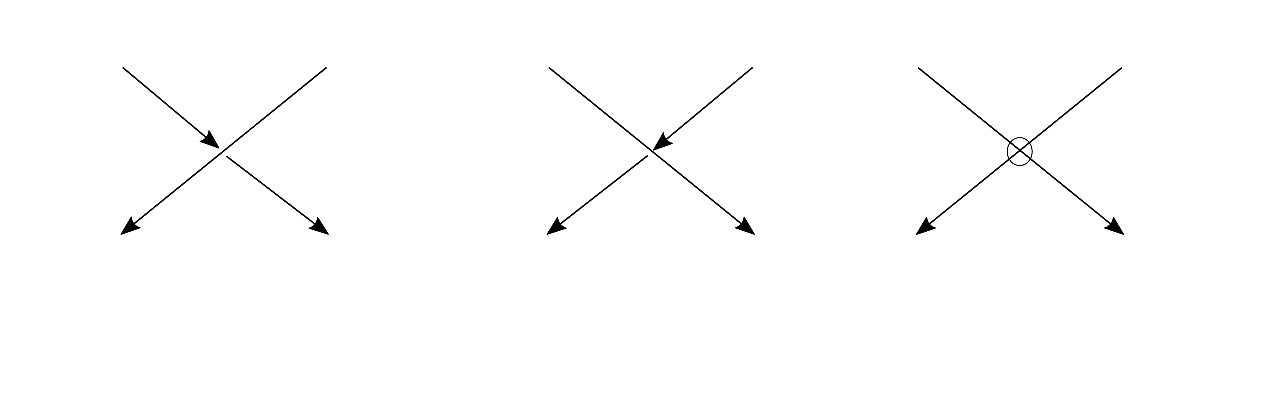
\includegraphics[width=\unitlength]{CrossingRelations.eps}}%
    \put(0.55065613,0.27402178){\color[rgb]{0,0,0}\makebox(0,0)[lt]{\lineheight{1.25}\smash{\begin{tabular}[t]{l}  $j^{th}$ component\end{tabular}}}}%
    \put(0.18308982,0.27402178){\color[rgb]{0,0,0}\makebox(0,0)[lt]{\lineheight{1.25}\smash{\begin{tabular}[t]{l}  $j^{th}$ component\end{tabular}}}}%
    \put(0.00042132,0.27402037){\color[rgb]{0,0,0}\makebox(0,0)[lt]{\lineheight{1.25}\smash{\begin{tabular}[t]{l}  $i^{th}$ component\end{tabular}}}}%
    \put(0.35275659,0.27402178){\color[rgb]{0,0,0}\makebox(0,0)[lt]{\lineheight{1.25}\smash{\begin{tabular}[t]{l}  $i^{th}$ component\end{tabular}}}}%
    \put(0.10442837,0.07458228){\color[rgb]{0,0,0}\makebox(0,0)[lt]{\lineheight{1.25}\smash{\begin{tabular}[t]{l}\\$c= b^{v_i}$,\\$d=b^{-v_i v_j^{-1}} a ^{v_j^{-1}} b^{v_i v_j^{-1}}$.\\\end{tabular}}}}%
    \put(0.4488261,0.04467432){\color[rgb]{0,0,0}\makebox(0,0)[lt]{\lineheight{1.25}\smash{\begin{tabular}[t]{l} $c=a b^{v_i} a^{-1}$,\\ $d=a^{v_j^{-1}}$.\end{tabular}}}}%
    \put(0.12078328,0.09067291){\color[rgb]{0,0,0}\makebox(0,0)[lt]{\lineheight{1.25}\smash{\begin{tabular}[t]{l}Positive\end{tabular}}}}%
    \put(0.4561577,0.09067127){\color[rgb]{0,0,0}\makebox(0,0)[lt]{\lineheight{1.25}\smash{\begin{tabular}[t]{l}Negative\end{tabular}}}}%
    \put(0.76997262,0.09067127){\color[rgb]{0,0,0}\makebox(0,0)[lt]{\lineheight{1.25}\smash{\begin{tabular}[t]{l}Virtual\end{tabular}}}}%
    \put(0.08044013,0.23389783){\color[rgb]{0,0,0}\makebox(0,0)[lt]{\lineheight{1.25}\smash{\begin{tabular}[t]{l}\textbf{a}\end{tabular}}}}%
    \put(0.23807669,0.22961827){\color[rgb]{0,0,0}\makebox(0,0)[lt]{\lineheight{1.25}\smash{\begin{tabular}[t]{l}\textbf{b}\end{tabular}}}}%
    \put(0.08044063,0.15755463){\color[rgb]{0,0,0}\makebox(0,0)[lt]{\lineheight{1.25}\smash{\begin{tabular}[t]{l}\textbf{c}\end{tabular}}}}%
    \put(0.23891552,0.15327667){\color[rgb]{0,0,0}\makebox(0,0)[lt]{\lineheight{1.25}\smash{\begin{tabular}[t]{l}\textbf{d}\end{tabular}}}}%
    \put(0.42327461,0.2338979){\color[rgb]{0,0,0}\makebox(0,0)[lt]{\lineheight{1.25}\smash{\begin{tabular}[t]{l}\textbf{a}\end{tabular}}}}%
    \put(0.4232753,0.1575563){\color[rgb]{0,0,0}\makebox(0,0)[lt]{\lineheight{1.25}\smash{\begin{tabular}[t]{l}\textbf{c}\end{tabular}}}}%
    \put(0.57932689,0.22961827){\color[rgb]{0,0,0}\makebox(0,0)[lt]{\lineheight{1.25}\smash{\begin{tabular}[t]{l}\textbf{b}\end{tabular}}}}%
    \put(0.58016445,0.15327667){\color[rgb]{0,0,0}\makebox(0,0)[lt]{\lineheight{1.25}\smash{\begin{tabular}[t]{l}\textbf{d}\end{tabular}}}}%
    \put(0.72284793,0.23390023){\color[rgb]{0,0,0}\makebox(0,0)[lt]{\lineheight{1.25}\smash{\begin{tabular}[t]{l}\textbf{a}\end{tabular}}}}%
    \put(0.87864283,0.15755863){\color[rgb]{0,0,0}\makebox(0,0)[lt]{\lineheight{1.25}\smash{\begin{tabular}[t]{l}\textbf{a}\end{tabular}}}}%
    \put(0.87776214,0.2296206){\color[rgb]{0,0,0}\makebox(0,0)[lt]{\lineheight{1.25}\smash{\begin{tabular}[t]{l}\textbf{b}\end{tabular}}}}%
    \put(0.72197109,0.153279){\color[rgb]{0,0,0}\makebox(0,0)[lt]{\lineheight{1.25}\smash{\begin{tabular}[t]{l}\textbf{b}\end{tabular}}}}%
  \end{picture}%
\endgroup%

\caption{Crossing relations.}\label{F: Crossings Relations}
\end{figure}

%%%%%%%%%%%%%%%%%%%%%%%%%%%%%%%%%%%%%%%%%%%%%%%%%%%%%%%%%%%%%%%%
\par
If $D'(L)$ is another diagram representing $L$, then $D_L$ and $D'(L)$ are equivalent under finite sequence of {\it generalized Reidemeister moves} shown in Figure \ref{F: CVReidMoves} upto planar isotopy. The following statement is an analogous to the case of classical link diagrams and is easy to prove.

\begin{proposition}
If $D_L$ and $D_L'$ are two diagrams of a virtual link $L$, then groups $G_M(D_L)$ and $G_M(D_L')$ are isomorphic. Hence $G_M(D_L)$ is an invariant of $L$.
\end{proposition}
We also note down the following result.
\begin{proposition}
Let $L$ be a virtual link, $D_L$ be its diagram, $\beta$ be a braid such that its closure $\hat{\beta}$ is equivalent to $L$, then $G_M(D_L) \cong G_{M}(\beta)$. Denote $G_M(L):=G_M(D_L)$.
\end{proposition}

\begin{remark}\label{R: one component link}
Let $\beta \in VB_n$ such that the closure of $\beta$ is a one component virtual link. Then $G_M(\beta) \cong G_{\tilde{\varphi_0}}(\beta)$, where $\tilde{\varphi_0}$ is Generalized Artin representation $($see Subsection \ref{SS: Generalized Artin representation}$)$.
\end{remark}

\begin{remark}
If we put all $v_i's$ equal to $1$ in $G_M(L)$, then we get a group $G_0(L)$ defined by L.~Kauffman \cite{Kauffman-1}.
\end{remark}

\subsection{Gauss diagram approach}\label{GaussDiagramsAndGroups}
A \textit{Gauss diagram} consists of finite number of circles oriented anticlockwise with finite number of signed arrows whose head and tail lie on circles. If head and tail of an arrow lie on the same circle, then we will call it a chord. For each virtual link diagram one can construct a Gauss diagram. There is one-to-one correspondence between virtual links and Gauss diagrams considered upto moves shown in Figure \ref{fig:GaussMoves}. See \cite{GPV-1, Kauffman-1, Petter-1} for more details.

\begin{figure}[H]
    $$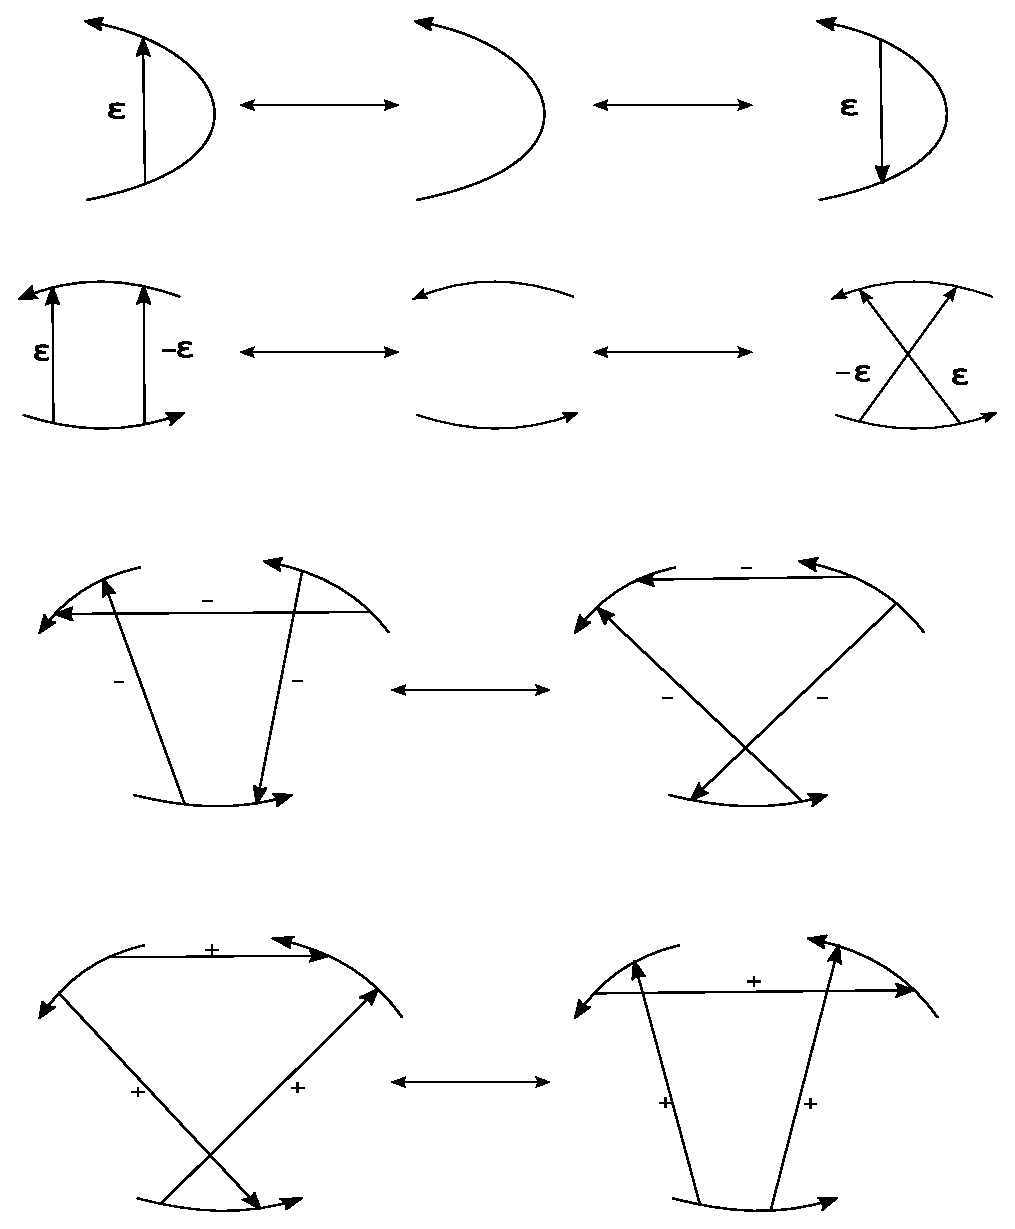
\includegraphics[width=10cm]{Rmoves.eps}$$
    \caption{Moves on Gauss diagrams corresponding to Reidemeister moves.}
    \label{fig:GaussMoves}
    \end{figure}

An advantage of using the representation $\varphi_M:VB_n \to \Aut(F_{n,n})$ over $\varphi: VB_n \to \Aut(F_{n,n})$ is that one can describe virtual link group $G_M(L)$ in terms of \textrm{Gauss diagram} as follows. Let $D$ be a Gauss diagram with $m$ circles corresponding to the virtual link $L$. Identify circles with numbers from $1$ to $m$, and add generator $v_i$, $1 \leq i \leq m$, with relations $v_i v_j =v_j v_i$ for $1 \leq i, j \leq m$. If we cut the circles at head and tail of each arrow, then circles of $D$ are divided into set of arcs. To each of these arcs there corresponds a generator of the group. Each arrow gives two relations under the following rules.
\begin{itemize}
\item If the sign of an arrow is $+1$, its tail is the final point of an arc labeled $b$ and initial point of an arc labeled $c$, where $b$ and $c$ lies on the $j^{th}$ circle, and its head is the final point of an arc labeled $a$ and the initial point of an arc labeled $d$, where $a$ and $d$ lies on the $i^{th}$ circle, then we assign the following relations to this arrow:
\begin{align*}
c&=b^{v_i},\\
d&=b^{-v_i v_j ^{-1}} a^{v_j ^{-1}} b ^{v_i v_j ^{-1}}.
\end{align*}
\item If the sign of an arrow is $-1$, its tail is the final point of an arc labeled $a$ and initial point of an arc labeled $d$, where $a$ and $d$ lies on the $i^{th}$ circle, and its head is the final point of an arc labeled $b$ and the initial point of an arc labeled $c$, where $b$ and $c$ lies on the $j^{th}$ circle, then we assign the following relations to this arrow:
\begin{align*}
c&=a b ^{v_i} a^{-1},\\
d&=a^{v_j^{-1}}.
\end{align*}
\end{itemize}
Denote the group assigned to $D$ using the above rules by $\pi_D$. Clearly, $\pi_D$ is an irreducible $C_m$-group. 
Notice that $\pi_D \cong G_M(L)$.


\medskip


\section{marked Gauss diagrams}\label{S: marked Gauss Diagrams}

In this section we will define and study Gauss diagrams with additional structure. We will extend the notion of virtual link group to these diagrams. 

\begin{definition}
A \textit{marked Gauss diagram} consists of finite number of circles oriented anticlockwise with finite number of signed arrows whose head and tail lie on circles, and finite number of signed nodes lying on circles and not attach to arrows. If head and tail of an arrow lie on the same circle, then we will call it a chord.
\end{definition}

Figure \ref{F: Example-1} has two $1$-circle marked Gauss diagrams and Figure \ref{F: Example-2} has a $3$-circle marked Gauss diagram.

\begin{figure}[H]
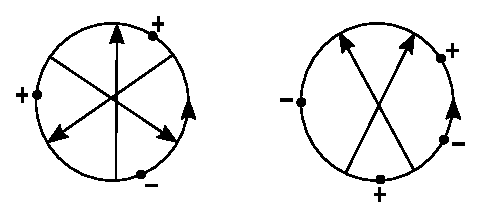
\includegraphics[width=5cm]{example-1.eps}
    \caption{Two $1$-circle marked Gauss diagrams.}
    \label{F: Example-1}
\end{figure}


\begin{figure}[H]
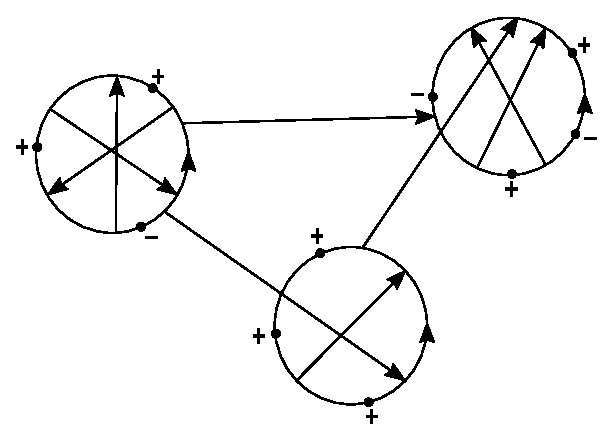
\includegraphics[width=5cm]{example-2.eps}
    \caption{A $3$-circle marked Gauss diagram.}
    \label{F: Example-2}
\end{figure}

We will consider marked Gauss diagrams upto the equivalence relation generated by finite sequence of moves shown in Figure \ref{fig:GaussMoves} and Figure \ref{F: AddGaussMoves}. In Figure \ref{F: AddGaussMoves}, moves involving arcs belong to $i^{th}$ circle in a given marked Gauss diagram. Moreover, moves in Figure \ref{fig:GaussMoves} and \ref{F: AddGaussMoves} will collectively be called \textit{marked Reidemeister moves}. 

\begin{figure}[H]
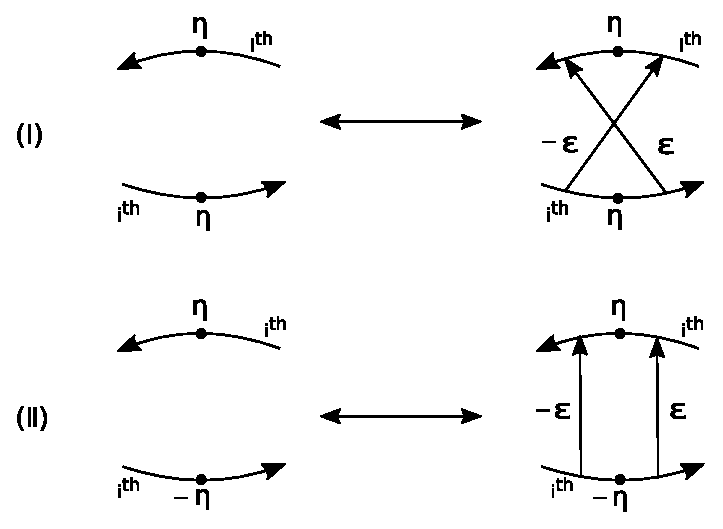
\includegraphics{GRmoves.eps}
\caption{Additional moves on marked Gauss diagrams.}
\label{F: AddGaussMoves}
\end{figure}


It is clear from Figure \ref{F: AddGaussMoves} that marked Gauss diagrams are {\it proper} generalization of Gauss diagrams, i.e., there is a canonical injective map from equivalence classes of Gauss diagrams to equivalence classes of marked Gauss diagrams.
\par

Now to each marked Gauss diagram we will associate a group as follows. Let $D$ be a marked Gauss diagram with $m$ circles. Identify circles with numbers from $1$ to $m$, and add generator $v_i$, $1 \leq i \leq m$, with relations $v_i v_j=v_jv_i$ for $1 \leq i, j \leq m$. Cut the circles at head and tail of each arrow and at node points. Then circles of $D$ are divided into set of arcs. To each of these arcs there corresponds a generator of the group. For each arrow we add two relations under the following rules.
\begin{itemize}
\item If the sign of an arrow is $+1$, its tail is the final point of an arc labeled $b$ and initial point of an arc labeled $c$, where $b$ and $c$ lies on the $j^{th}$ circle, and its head is the final point of an arc labeled $a$ and the initial point of an arc labeled $d$, where $a$ and $d$ lies on the $i^{th}$ circle, then we assign the following relations to this arrow:
\begin{align*}
c&=b^{v_i}\\
d&=b^{-v_i v_j ^{-1}} a^{v_j ^{-1}} b ^{v_i v_j ^{-1}}.
\end{align*}
\item If the sign of an arrow is $-1$, its tail is the final point of an arc labeled $a$ and initial point of an arc labeled $d$, where $a$ and $d$ lies on the $i^{th}$ circle, and its head is the final point of an arc labeled $b$ and the initial point of an arc labeled $c$, where $b$ and $c$ lies on the $j^{th}$ circle, then we assign the following relations to this arrow:
\begin{align*}
c&=a b ^{v_i} a^{-1}\\
d&=a^{v_j^{-1}}.
\end{align*}
\end{itemize}
And for each node we add one relation as follows. If the node over the circle $i$ is the final point of arc labeled $x$ and initial point of arc labeled $y$, then we add relation $y=x^{v_i^{\eta}}$ where $\eta$ is sign of the node. This group will be denoted by $\Pi_D$ and is called the {\it group of the marked Gauss diagram}. Clearly, $\Pi_D$ is an irreducible $C_m$-group. One can check that the group $\Pi_D$ is invariant under marked Reidemeister moves. Moreover, if $D$ is a Gauss diagram, then $\Pi_D \cong \pi_D$. Therefore, the notion of a virtual link group is extended to marked Gauss diagrams.
\par

\begin{proposition}
Number of nodes, and sum and product of sign of nodes in a given marked Gauss diagram are invariant under marked Reidemeister moves.
\end{proposition}
\begin{proof}
It is easy to observe that under any move given in Figure \ref{fig:GaussMoves} and Figure \ref{F: AddGaussMoves}, the number of nodes, and sum and product of sign of nodes do not change.
\end{proof}

\begin{figure}[H]
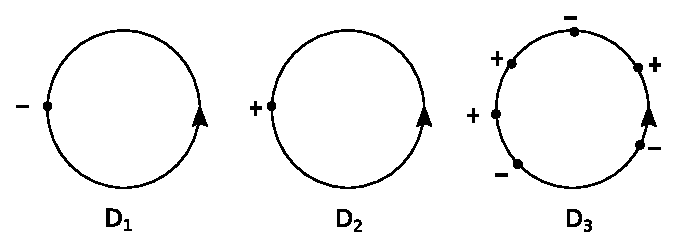
\includegraphics{nodes-1.eps}
\caption{Marked Gauss diagrams with isomorphic groups.}
\label{fig:general-Gauss-diagrams-with-isomorphic-group}
\end{figure}

\begin{example}
In Figure \ref{fig:general-Gauss-diagrams-with-isomorphic-group}, $D_1$ has presentation $\langle a,v ~~||~~a=a^{v^{-1}} \rangle$
and $D_2$ has presentation $\langle b,v ~~||~~b=b^{v} \rangle$. Clearly $\Pi_{D_1} \cong \Pi_{D_2} \cong \mathbb{Z}^2.$ But these diagrams $D_1$ and $D_2$ are not equivalent as the sum of sign of nodes are not equal. Moreover, in $D_3$, we have equal number of positive and negative nodes and no chords, thus $\Pi_{D_3} \cong \mathbb{Z}*\mathbb{Z}$.
\end{example}

Let $T$ denotes a Gauss diagram corresponding to a trivial knot. Then we have a following result.

\begin{proposition}
There exist infinitely many marked Gauss diagrams with associated group isomorphic to $\Pi_T = \mathbb{Z}* \mathbb{Z}$.
\end{proposition}
\begin{proof}
Let $D$ be a $1$-circle marked Gauss diagram with equal number of positive and negative nodes and no chords. Then clearly, $\Pi_D \cong \Pi_T = \mathbb{Z} * \mathbb{Z}$. 
\end{proof}

\begin{proposition}
The group associated to a given $1$-circle marked Gauss diagram is an irreducible $C_1$-group of deficiency $1$ or $2$ and its second homology group is cyclic.
\end{proposition}




\begin{proof}
Let $D$ be a $1$-circle marked Gauss diagram and $\Pi_D$ be the group associated to it having deficiency $d$. Then the group $\Pi_D$ has a presentation $\mathcal{P}$ with $n+d$ generators $x_i$ and $n$ relations $r_j$. Let $X$ be the presentation complex of $\mathcal{P}$. The cellular chain complex of $X$ is

$$\ldots\to 0\to \mathbb{Z} ^n \stackrel{\partial_2}{\to} \mathbb{Z}^{n+d}
\stackrel{\partial_1}{\to}\mathbb{Z}.$$

Since $\Pi_D$ is an irreducible $C_1$-group and $\partial_1=0$, we have $d \leq 2$. Thus $\Pi_D$ has deficiency either $1$ or $2$.
Similarly, $H_2(X)$ is $0$ for $d=2$ and $\mathbb{Z}$ for $d=1$. Moreover, $X$ is the $2$-skeleton of Eilenberg-MacLane space $K(\Pi_D,1)$, hence $H_2(\Pi_D)$ is cyclic.
\end{proof}

\begin{corollary}
Every virtual knot group has deficiency $1$ or $2$, and its second homology group is cyclic.
\end{corollary}

\begin{example}
Let $K$ be a classical knot. Then by Remark \ref{R: one component link}, \cite[Proposition 4]{BB-1}, and Theorem \ref{isomorphism-of-G-and-G_M}, $G_M(K) \cong G_0(K) * \langle v \rangle$ and hence is of deficiency $2$, and $H_2\big(G_M(K)\big)=0$.
\end{example}

\begin{example}\label{ex:Group-of-general-Gauss-diagram}
Let $G$ be an irreducible $C$-group such that $H_2(G) \neq 0$ and $G^*=G * \langle v \rangle$ be the free product of $G$ and $\langle v \rangle$. Since $H_2(G^*)=H_2(G) \oplus H_2(\mathbb{Z})=H_2(G)$, $H_2(G^*) \neq 0$. In Section \ref{S: Realization-of-irreducible $C_1$-group}, we shall show that $G^*$ is the group of some marked Gauss diagram. Thus $G^*$ is the group of a marked Gauss diagram with deficiency $1$. In \cite{Gordon-1}, C. Gordon gave a family of irreducible $C$-groups whose second homology groups are $\mathbb{Z}$, and in \cite{BMS-1}, A. Brunner, E. Mayland, and J. Simon constructed an irreducible $C$-group with second homology group of order $2$.
\end{example}


\section{Marked virtual link diagrams}\label{S: Marked virtual link diagrams}
In this section we give an interpretation of marked Gauss diagrams in terms of diagrams which nearly look like virtual link diagrams.
\par

Let $G=(V,E)$ be a {\it directed graph}, where $V$ denotes the set of vertices and $E$ denotes the set of directed edges. A {\it diwalk} 
is an alternating sequence of vertices and edges $v_0, e_1, v_1, \ldots, v_{n-1}, e_n, v_n$ with edge $e_i$ directed from $v_{i-1} $ to $v_i$, $v_0, v_1, \ldots, v_n \in V$ and $e_1, e_2, \ldots e_n \in E$ . A {\it directed cycle} is a diwalk in which all vertices except the first and last are different. From now onward by a {\it cycle} we mean directed cycle.
\par
In the paper \cite{BH-1}, L. Beineke and F. Harary introduced {\it marked graphs}. A directed graph is called {\it marked} if each vertex is assigned either positive or negative sign. We define {\it marked cycles} as a marked graph consisting only of cycles and no cycle shares a common vertex with another cycle. See Figure \ref{F: Illustration of marked cycles}.
\par
 
In \cite{FM-1}, T. Fleming and B. Mellor defined {\it virtual spatial graph diagram} as a generic immersion of directed graph $G$ in $\mathbb{R}^2$ where the double points are either classical crossings or virtual crossings. Now we will define {\it marked virtual spatial graph diagram} and {\it marked virtual link diagrams.}
\begin{definition}
A {\it marked virtual spatial graph diagram} is a virtual spatial graph diagram with each vertex designated as being either positive or negative, i.e., generic immersion of marked graph in $\mathbb{R}^2$ with information of virtual and classical crossings.
\end{definition}

\begin{definition}
A {\it marked virtual link diagram} is generic immersion of marked cycles in $\mathbb{R}^2$ with information of virtual and classical crossings. If it is one component diagram, then we will call it as {\it marked virtual knot diagram}.
\end{definition}

It is clear that for a given marked Gauss diagram one can draw a marked virtual link diagram and other way round is also true. See Figure \ref{F: MGDandMVLD}.

\begin{figure}[H]
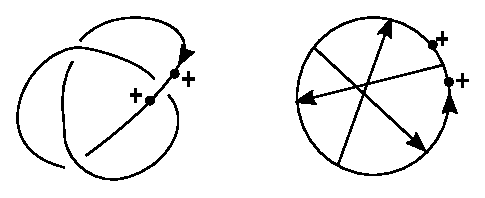
\includegraphics[width=7cm]{MGDandMVLD.eps}
\caption{Marked virtual knot diagram and its marked Gauss diagram.} \label{F: MGDandMVLD}
\end{figure}

We say two marked virtual link diagrams are {\it equivalent} if they are related by a finite sequence of moves shown in Figure \ref{F: CVReidMoves} and Figure \ref{F: MixedReidMoves}. It is clear that there is one-to-one correspondence between equivalence classes of marked Gauss diagrams and equivalence classes of marked virtual link diagrams. In Figure \ref{F: ForbiddenReidMoves}, we add forbidden moves on marked virtual link diagrams. In $($F\RNum{2}$)$ move, $i^{th}$-component is not equal to $j^{th}$-component and $\epsilon \neq \eta$.

\begin{figure}[H]
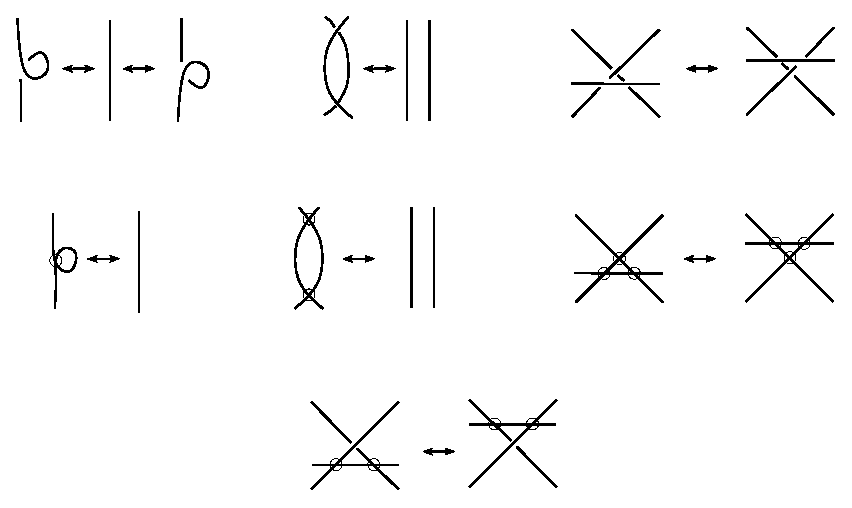
\includegraphics{CVReidMoves-1.eps}
\caption{Generalized Reidemeister moves.} \label{F: CVReidMoves}
\end{figure}

\begin{figure}[H]
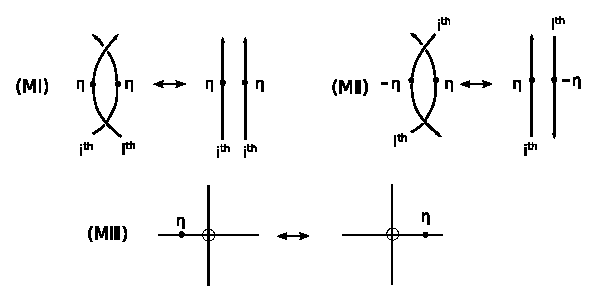
\includegraphics{MixedReidMoves-1.eps}
\caption{Mixed Reidemeister moves for marked virtual links.}\label{F: MixedReidMoves}
\end{figure}

\begin{figure}[H]
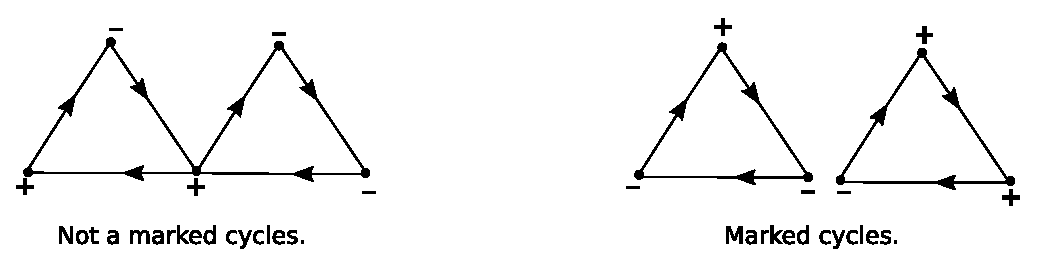
\includegraphics[width=12cm]{graphs.eps}
\caption{Illustration of marked cycles.}\label{F: Illustration of marked cycles}
\end{figure}

\begin{figure}[H]
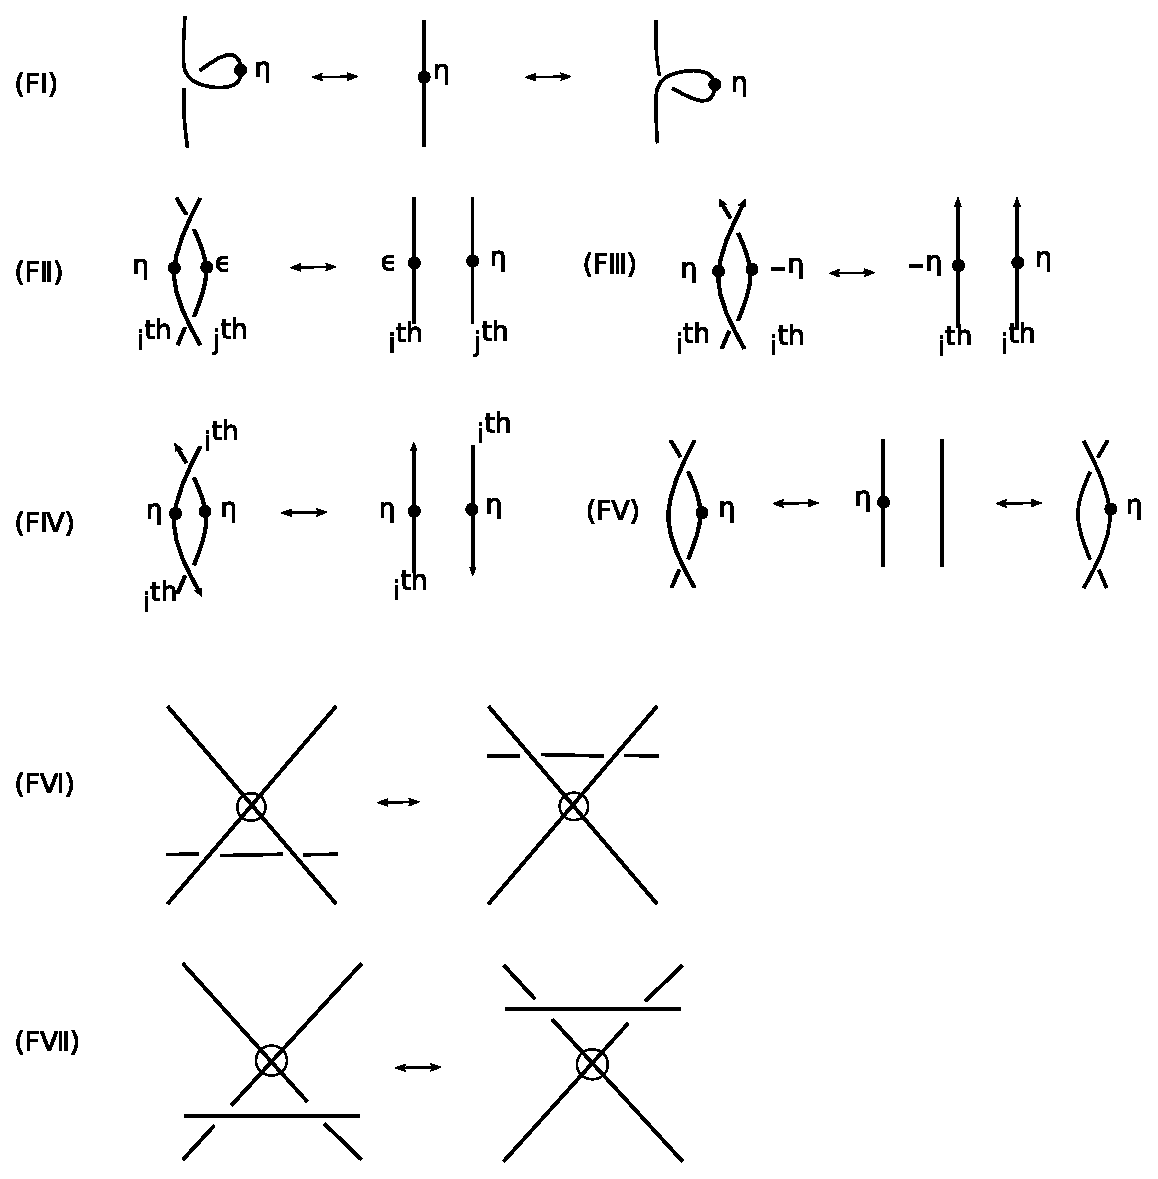
\includegraphics[width=9cm]{ForbiddenReidMoves.eps}
\caption{Forbidden Reidemeister moves for marked virtual links.} \label{F: ForbiddenReidMoves}
\end{figure}

Let $D$ be a marked Gauss diagram and $D_L$ a corresponding marked virtual link diagram. Then the group $\Pi_D$ can be defined from $D_L$ using the relations given in Figure \ref{F: Marked Crossings Relations}.

\begin{figure}[H]
\def\svgwidth{14.5cm}
\begingroup%
  \makeatletter%
  \providecommand\color[2][]{%
    \errmessage{(Inkscape) Color is used for the text in Inkscape, but the package 'color.sty' is not loaded}%
    \renewcommand\color[2][]{}%
  }%
  \providecommand\transparent[1]{%
    \errmessage{(Inkscape) Transparency is used (non-zero) for the text in Inkscape, but the package 'transparent.sty' is not loaded}%
    \renewcommand\transparent[1]{}%
  }%
  \providecommand\rotatebox[2]{#2}%
  \newcommand*\fsize{\dimexpr\f@size pt\relax}%
  \newcommand*\lineheight[1]{\fontsize{\fsize}{#1\fsize}\selectfont}%
  \ifx\svgwidth\undefined%
    \setlength{\unitlength}{595.24848652bp}%
    \ifx\svgscale\undefined%
      \relax%
    \else%
      \setlength{\unitlength}{\unitlength * \real{\svgscale}}%
    \fi%
  \else%
    \setlength{\unitlength}{\svgwidth}%
  \fi%
  \global\let\svgwidth\undefined%
  \global\let\svgscale\undefined%
  \makeatother%
  \begin{picture}(1,0.30343312)%
    \lineheight{1}%
    \setlength\tabcolsep{0pt}%
    \put(0,0){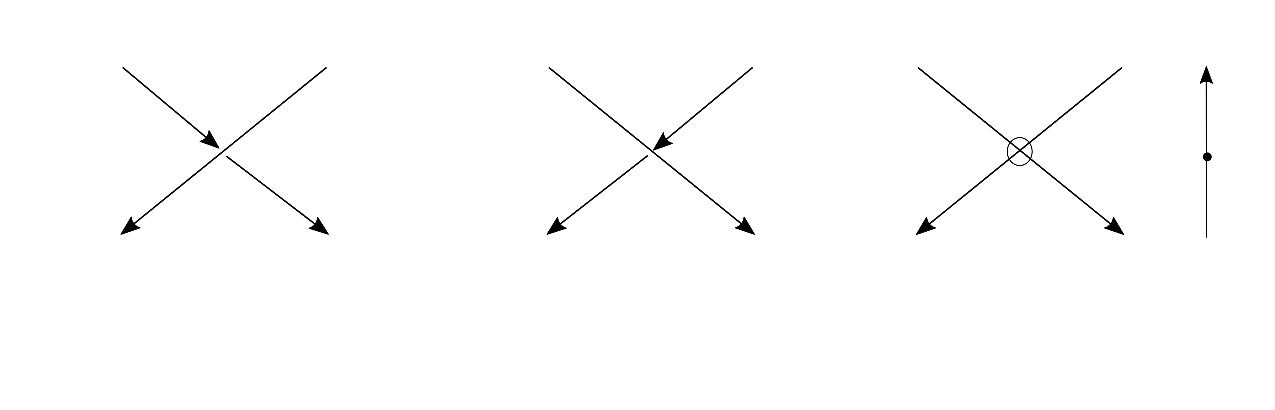
\includegraphics[width=\unitlength]{MarkedLinkRelations.eps}}%
    \put(0.55065613,0.27402178){\color[rgb]{0,0,0}\makebox(0,0)[lt]{\lineheight{1.25}\smash{\begin{tabular}[t]{l}  $j^{th}$ component\end{tabular}}}}%
    \put(0.18308982,0.27402178){\color[rgb]{0,0,0}\makebox(0,0)[lt]{\lineheight{1.25}\smash{\begin{tabular}[t]{l}  $j^{th}$ component\end{tabular}}}}%
    \put(0.01092718,0.27402033){\color[rgb]{0,0,0}\makebox(0,0)[lt]{\lineheight{1.25}\smash{\begin{tabular}[t]{l}  $i^{th}$ component\end{tabular}}}}%
    \put(0.37039633,0.27402178){\color[rgb]{0,0,0}\makebox(0,0)[lt]{\lineheight{1.25}\smash{\begin{tabular}[t]{l}  $i^{th}$ component\end{tabular}}}}%
    \put(0.10442837,0.07458228){\color[rgb]{0,0,0}\makebox(0,0)[lt]{\lineheight{1.25}\smash{\begin{tabular}[t]{l}\\$c= b^{v_i}$,\\$d=b^{-v_i v_j^{-1}} a ^{v_j^{-1}} b^{v_i v_j^{-1}}$.\\\end{tabular}}}}%
    \put(0.4488261,0.04467432){\color[rgb]{0,0,0}\makebox(0,0)[lt]{\lineheight{1.25}\smash{\begin{tabular}[t]{l} $c=a b^{v_i} a^{-1}$,\\ $d=a^{v_j^{-1}}$.\end{tabular}}}}%
    \put(0.12078328,0.09067291){\color[rgb]{0,0,0}\makebox(0,0)[lt]{\lineheight{1.25}\smash{\begin{tabular}[t]{l}Positive\end{tabular}}}}%
    \put(0.4561577,0.09067127){\color[rgb]{0,0,0}\makebox(0,0)[lt]{\lineheight{1.25}\smash{\begin{tabular}[t]{l}Negative\end{tabular}}}}%
    \put(0.76997262,0.09067127){\color[rgb]{0,0,0}\makebox(0,0)[lt]{\lineheight{1.25}\smash{\begin{tabular}[t]{l}Virtual\end{tabular}}}}%
    \put(0.08044013,0.23389783){\color[rgb]{0,0,0}\makebox(0,0)[lt]{\lineheight{1.25}\smash{\begin{tabular}[t]{l}\textbf{a}\end{tabular}}}}%
    \put(0.23807669,0.22961827){\color[rgb]{0,0,0}\makebox(0,0)[lt]{\lineheight{1.25}\smash{\begin{tabular}[t]{l}\textbf{b}\end{tabular}}}}%
    \put(0.08044063,0.15755463){\color[rgb]{0,0,0}\makebox(0,0)[lt]{\lineheight{1.25}\smash{\begin{tabular}[t]{l}\textbf{c}\end{tabular}}}}%
    \put(0.23891552,0.15327667){\color[rgb]{0,0,0}\makebox(0,0)[lt]{\lineheight{1.25}\smash{\begin{tabular}[t]{l}\textbf{d}\end{tabular}}}}%
    \put(0.42327461,0.2338979){\color[rgb]{0,0,0}\makebox(0,0)[lt]{\lineheight{1.25}\smash{\begin{tabular}[t]{l}\textbf{a}\end{tabular}}}}%
    \put(0.4232753,0.1575563){\color[rgb]{0,0,0}\makebox(0,0)[lt]{\lineheight{1.25}\smash{\begin{tabular}[t]{l}\textbf{c}\end{tabular}}}}%
    \put(0.57932689,0.22961827){\color[rgb]{0,0,0}\makebox(0,0)[lt]{\lineheight{1.25}\smash{\begin{tabular}[t]{l}\textbf{b}\end{tabular}}}}%
    \put(0.58016445,0.15327667){\color[rgb]{0,0,0}\makebox(0,0)[lt]{\lineheight{1.25}\smash{\begin{tabular}[t]{l}\textbf{d}\end{tabular}}}}%
    \put(0.72284793,0.23390023){\color[rgb]{0,0,0}\makebox(0,0)[lt]{\lineheight{1.25}\smash{\begin{tabular}[t]{l}\textbf{a}\end{tabular}}}}%
    \put(0.87864283,0.15755863){\color[rgb]{0,0,0}\makebox(0,0)[lt]{\lineheight{1.25}\smash{\begin{tabular}[t]{l}\textbf{a}\end{tabular}}}}%
    \put(0.87776214,0.2296206){\color[rgb]{0,0,0}\makebox(0,0)[lt]{\lineheight{1.25}\smash{\begin{tabular}[t]{l}\textbf{b}\end{tabular}}}}%
    \put(0.72197109,0.153279){\color[rgb]{0,0,0}\makebox(0,0)[lt]{\lineheight{1.25}\smash{\begin{tabular}[t]{l}\textbf{b}\end{tabular}}}}%
    \put(0.97022022,0.11733835){\color[rgb]{0,0,0}\makebox(0,0)[lt]{\lineheight{1.25}\smash{\begin{tabular}[t]{l}\textbf{a}\end{tabular}}}}%
    \put(0.97156509,0.24336541){\color[rgb]{0,0,0}\makebox(0,0)[lt]{\lineheight{1.25}\smash{\begin{tabular}[t]{l}\textbf{b}\end{tabular}}}}%
    \put(0.96695724,0.18485935){\color[rgb]{0,0,0}\makebox(0,0)[lt]{\lineheight{1.25}\smash{\begin{tabular}[t]{l}$\eta$\end{tabular}}}}%
    \put(0.89039861,0.28456484){\color[rgb]{0,0,0}\makebox(0,0)[lt]{\lineheight{1.25}\smash{\begin{tabular}[t]{l}  $i^{th}$ component\end{tabular}}}}%
    \put(0.9105975,0.04469159){\color[rgb]{0,0,0}\makebox(0,0)[lt]{\lineheight{1.25}\smash{\begin{tabular}[t]{l}$b=a^{v_i^{\eta}}.$\end{tabular}}}}%
  \end{picture}%
\endgroup%

\caption{Crossing relations in virtual link diagrams.}\label{F: Marked Crossings Relations}
\end{figure}


\medskip

\section{Realization of irreducible $C_1$-groups}\label{S: Realization-of-irreducible $C_1$-group}
In this section we will show that every irreducible $C_1$-group is the group of some $1$-circle marked Gauss diagram.

\begin{definition}\label{cyclic irreducible $C_1$-presentation}
A \textit{cyclic irreducible $C_1$-presentation} is an irreducible $C_1$-presentation of the form
$$
\langle x_1, x_2, \ldots, x_n,v~~||~~r_1, r_2, \ldots , r_n \rangle,
$$
where the $j^{th}$ relation $r_j$ is of the form $x_{j+1} ^{-1} x_j ^{w_j}$ for $j \in \mathbb{Z}_n$, and some word $w_j$ in alphabets $x_1^{\pm 1}, x_2^{\pm 1}, \ldots , x_n^{\pm 1}, v^{\pm 1}$.
\end{definition}

\begin{definition}\label{realizable irreducible $C_1$-presentation}
A \textit{realizable irreducible $C_1$-presentation} is a cyclic irreducible $C_1$-presentation where $w_j$ belongs to $\{ v^{-\epsilon}x_1^{\epsilon}, \ldots, v^{-\epsilon}x_n^{\epsilon}, v^{\epsilon}~~||~~\epsilon=\pm 1 \}$. If $w_k=v^{-1}x_p$, then $x_{p+1}=x_p^{v}$ and if $w_k=vx_p^{-1}$, then $x_{p+1}=x_p^{v^{-1}}$. Moreover, $w_j \neq v^{-\epsilon} x_p^{\epsilon}, v^{-\epsilon} x_k^{\epsilon}$ where $k \neq j$.

\end{definition}

In the following result we have used the same technique as described in \cite[Lemma 2]{Kim-1}.

\begin{proposition}\label{irreducible $C_1$-presentation-to-cyclic irreducible $C_1$-presentation}
Any irreducible $C_1$-presentation can be transformed to a cyclic irreducible $C_1$-presentation.
\end{proposition}
\begin{proof}
Let $\mathcal{P}= \langle x_1, \ldots, x_n,v ~~||~~r_1, \ldots, r_m \rangle$ be an irreducible $C_1$-presentation. Either $m=n$ or $n-1$. If $m=n-1$, we will add one more relation $r_{m+1}=r_m$ and thus we can assume $m=n$. Consider a graph $\Gamma$ associated to presentation $\mathcal{P}$ as defined in Section \ref{S: prelim}. If $\Gamma$ has two edges $e_j^i$ and $e_k^j$ meeting at the vertex $x_j$, then there are relations $x_i^{-1}x_j^{w_{j,i}}$ and $x_j^{-1} x_k^{w_{k,j}}$ in $\mathcal{P}$. Removing relation $x_i^{-1}x_j^{w_{j,i}}$ and adding relation $x_i^{-1}x_k^{w_{k,j}w_{j,i}}$ corresponds to an operation on $\Gamma$ as removing edge $e_j^i$ and adding $e_k^i$. Clearly this operation does not change the underlying group. Since $\Gamma$ is a connected graph and number of edges is equal to number of vertices, $\Gamma$ has exactly one cycle $C$. If length $l(C)$ of cycle $C$ is $n$, then $\mathcal{P}$ is cyclic irreducible $C_1$-presentation and if not, then since $\Gamma$ is connected, there is an edge $e_j ^i$ such that $x_i$ is in $C$ and $x_j$ is not in $C$. Using the above operation we get a graph $\Gamma '$ with cycle $C'$ containing all vertices of $C$ and $x_j$. Clearly $l(C')=l(C)+1$. Thus after finitely many steps we will get a graph with cycle length $n$ and consequently, a cyclic irreducible $C_1$-presentation.
\end{proof}


\begin{proposition}\label{cyclic irreducible $C_1$-presentation-to-realizable-irreducible $C_1$-presentation}
Every cyclic irreducible $C_1$-presentation can be transformed to a realizable irreducible $C_1$-presentation.
\end{proposition}
\begin{proof}
On a given cyclic irreducible $C_1$-presentation $\mathcal{P}$ perform the following steps in order and we will get a realizable irreducible $C_1$-presentation.
\begin{itemize}
\item\label{Step1} \textit{Step $1$:} Make each $w_j$ one of the letter in $\{ x_1^{\pm 1}, \ldots, x_n^{\pm 1}, v^{\pm 1} \}$. For example, let $w_j= x_4 x_3 v^{-1}$ and $r_j= x_{j+1}^{-1}x_j^{w_j}$. Then introduce two more generators say $x_j'$ and $x_j''$, remove the relation $r_j$ and add three more relations $x_j'^{-1} x_j^{x_4}$, ${x_j''}^{-1} x_j'^{x_3}$ and $x_{j+1}^{-1}{x_j''}^{v^{-1}}$. Now we get a new cyclic irreducible $C_1$-presentation presenting the same group.

\vspace{.5mm}
\item \textit{Step $2$:} Let $r_j=x_{j+1}^{-1} x_j^{x_j ^{\epsilon}}$ in cyclic irreducible $C_1$-presentation $\mathcal{P}$. Remove the relation $r_j$ and add two generators $x_j',x_j''$ and relations $x_j'=x_j^{v^{\epsilon}}$,
$x_j''=x_j'^{v^{-\epsilon}}$, $x_{j+1}=x_j''^{x_j^\epsilon}$. 

\vspace{.5mm}
\item \textit{Step $3$:} If $r_j=x_{j+1}x_j^{x_k^{\epsilon}}$ and $x_k \neq x_j$, then remove the relations $r_j$ and $r_k=x_{k+1}x_k^{w_k}$, add three generators $x_{k,1}, x_{k,2}, X_j$, five relations $x_{k,1}=x_k^{v^{\epsilon}}, x_{k,2}=x_{k,1}^{v^{-\epsilon}}, X_j=x_j^{v^{\epsilon}},x_{j+1}=X_j^{v^{-\epsilon}x_k^{\epsilon}}, x_{k+1}=x_{k,2}^{w_k}$. Moreover, replace $x_k$ by $x_{k,2}$ in words $w_i$ in presentation $\mathcal{P}$ for $i > j$. Do this step in the increasing order on relations.

\end{itemize}

\end{proof}

\begin{corollary}\label{irreducible $C_1$-presentation-to-realizable-irreducible $C_1$-presentation}
Any irreducible $C_1$-presentation can be transformed to a realizable irreducible $C_1$-presentation.
\end{corollary}


\begin{theorem}\label{RealizationOfirreducible $C_1$-presentation}
Any irreducible $C_1$-group can be realized as the group of a marked Gauss diagram.
\end{theorem}
\begin{proof}
Let $\mathcal{P}$ be an irreducible $C_1$-presentation of a given irreducible $C_1$-group. By Corollary \ref{irreducible $C_1$-presentation-to-realizable-irreducible $C_1$-presentation} we can assume $\mathcal{P}$ is a realizable irreducible $C_1$-presentation having $n+1$ generators $x_1, \ldots x_n, v$ and $n$ relations $r_1, \ldots, r_n$. Now take a circle with anticlockwise orientation and mark $n$ points on it, dividing the circle into $n$ arcs. Label arcs as $x_1, \ldots, x_n$ successively in anticlockwise direction. Now do the following steps based on the type of relation.
\begin{itemize}
\item If $r_j = x_{j+1} ^{-1} x_j ^{v^{-\epsilon} x_k ^{\epsilon}}$, then attach a chord whose tail lies on the point joining arcs $x_k$ and $x_{k+1}$ and head on the point joining $x_j$ and $x_{j+1}$ arc. Assign sign $\epsilon$ to the chord.
\item If $r_j = x_{j+1}^{-1} x_j ^{v^{\epsilon}}$ and there is no relation of the type $x_{k+1}=x_k^{v^{-\epsilon} x_j^{\epsilon}}$ then put a node with $\epsilon$ sign on the point joining arcs $x_j$ and $x_{j+1}$.
\end{itemize}
One can check that the group of this marked Gauss diagram is the group corresponding to the presentation $\mathcal{P}$.
\end{proof}

Using the above result it is clear that the group $G^*$ in the Example \ref{ex:Group-of-general-Gauss-diagram} corresponds to some marked Gauss diagram $D$.

\section{Peripheral subgroup and peripheral structure}\label{S: Peripheral subgroup and peripheral structure}
It is well known that the fundamental group with the peripheral structure of a classical knot is a complete invariant of unoriented classical knots. For virtual knots one can define group system $($\cite{Kauffman-1, GPV-1, Kim-1, BB-1}$)$ but it is not a complete invariant. For example, if $K$ is the Kishino knot, then $(G_{\varphi_0}(K); (m,l))$ defined in \cite{BB-1} does not distinguish it from the trivial knot. In this section we will extend the notion of \textit{meridian}, \textit{longitude}, \textit{peripheral subgroup} and \textit{peripheral structure} to marked Gauss diagrams.
\par

Fix a base point on a circle of given marked Gauss diagram such that it does not lie on the end points of arrows and nodes. Let us assume we are on the $k^{th}$ circle. Then fix meridian $m_k$ to be the generator corresponding to the arc over which base point lies. Now we will describe how to write longitude $l_k$ for meridian $m_k$. Start moving along the circle from the base point in anticlockwise direction and write $v_t^{\epsilon}$ when passing the tail of an arrow whose sign is $\epsilon$ and head lies on $t^{th}$ circle, and
when passing the head of an arrow we use the following rule:
\begin{itemize}
\item if the sign of arrow is $+1$ write $v_n^{-1} x_i^{v_k v_n ^{-1}}$, where the head of arrow lies on $k^{th}$ circle, and the tail on $n^{th}$ circle and is the end point of $x_i$ labeled arc;

\item if the sign of the arrow is $-1$ write $v_n x_i ^{-1}$, where the tail of the arrow lies on the $n^{th}$ circle and is the end point of $x_i$ labeled arc;
\end{itemize}
And when we pass a node we write $v_{k}^{\epsilon}$ where $\epsilon$ is the sign of the node. On arriving at the base point we write $m_k^{-\alpha}$, where $\alpha$ is the sum of the sign of arrows whose head lies on the $k^{th}$ circle.
\par 

\begin{remark}
From now onward through out the paper by a marked Gauss diagram we mean $1$-circle marked Gauss diagram.
\end{remark}


\par
Let $D$ be a given marked Gauss diagram, $m$ a meridian and $l$ the corresponding longitude. A \textit{peripheral pair} of a marked Gauss diagram $D$ is the pair $(m, l)$ and the \textit{peripheral subgroup} corresponding to the meridian $m$ of $D$ is the subgroup of $\Pi_D$ generated by $m$ and $l$.
The pairs $(m,l)$ and $(m',l')$ are said to be \textit{conjugate} if there is an element $g$ in the group $\Pi_D$ such that $m'=m^g$ and $l'=l^g$. The \textit{peripheral structure} is the conjugacy class of a peripheral pair of $D$.
\par
Now we will prove that the peripheral structure of a marked Gauss diagram $D$ is unique and invariant under the marked Reidemeister moves.
Let $\Pi_D= \langle x_1, \ldots, x_n, v~~||~~r_1=x_2^{-1}x_1^{w_1}, \ldots, r_n=x_1^{-1}x_n^{w_n} \rangle$ be a presentation of $\Pi_D$ written down as per described in Section \ref{S: marked Gauss Diagrams}. If $x_1$ is a meridian of $D$, then $l=w_1\ldots w_n x_1^{-\alpha}$ is the corresponding longitude, where $\alpha$ is the sum of sign of chords in diagram $D$.

\begin{proposition}
The peripheral pair and the peripheral subgroup of a marked Gauss diagram are unique upto conjugacy and thus peripheral structure is well defined. Moreover, the peripheral structure is invariant under the marked Reidemeister moves.
\end{proposition}
\begin{proof}
Let $D$ be a marked Gauss diagram and choose two meridians $m_1$, $m_2$ corresponding to two different arcs of $D$. By construction of the group $\Pi_D$ there exist $g_1$ and $g_2$ in $\Pi_D$ such that $m_1=m_2^{g_2}$, $m_2=m_1^{g_1}$ and $l_1=g_1g_2m_1^{-\alpha}$, $l_2=g_2g_1m_2^{-\alpha}$, where $l_1$ and $l_2$ are longitudes corresponding to meridians $m_1$ and $m_2$, respectively. Now it is easy to see that $l_2=l_1^{g_1}$ and so $(m_1, l_1)^{g_1}=(m_2,l_2)$. Thus the peripheral pair and peripheral subgroup of $D$ are unique upto conjugacy and hence peripheral structure of $D$ is independent of choice of meridian. Now the invariance of peripheral structure under marked Reidemeister moves can be checked easily.
\end{proof}

\begin{proposition}
Peripheral subgroup of $\Pi_D$ is abelian.
\end{proposition}
\begin{proof}
By the previous proposition it is sufficient to prove that the subgroup generated by $x_1$ and the corresponding longitude $l=w_1 \ldots w_n x_1^{-\alpha}$ is abelian. From the relations in the presentation of $\Pi_D$ we have $x_1=x_1^{w_1 \ldots w_n}$ and thus meridian $x_1$ commutes with the longitude $l$.
\end{proof}

Let $G$ be a group with irreducible $C_1$-presentation $\mathcal{P}=\langle x_1, \ldots, x_n, v~~||~~r_1, \ldots, r_m \rangle$, and $g \in G$. Then $G_v$ denotes the group $\langle x_1, \ldots, x_n, v~~||~~r_1, \ldots, r_m, v \rangle $ and $g_v$  denotes the image of $g$ in $G_v$. It is easy to observe that for any marked Gauss diagram $D$, the image $l_v$ of longitude $l$ belongs to the commutator subgroup of ${\Pi_D}_v$.

\begin{theorem}\label{sufficiency-of-longitude}
Let $G$ be a group with irreducible $C_1$-presentation $\langle x_1, \ldots, x_n, v~~||~~r_1, \ldots, r_{n-1} \rangle$ and $l$ an element of $G$. If the image of $l$ in $G_v$ belongs to the commutator subgroup of $G_v$ and $l$ commutes with some conjugate of $x_1$ say $x_0$, then $G$ is the group of a marked Gauss diagram with peripheral pair $(x_0, l)$.
\end{theorem}

\begin{proof}
Since $x_0$ is conjugate to $x_1$, there exist some $w$ in $G$ such that $r_0:=x_1^{-1}x_0^{w}=1$. Thus $\mathcal{P}=\langle x_0,x_1, \ldots, x_n, v~~||~~r_0,r_1, \ldots, r_{n-1} \rangle$ presents the group $G$. We may assume that each relation in $\mathcal{P}$ is of the form $r_i=x_{i+1}^{-1}x_i^{w_i}$, $i=0,1, \ldots, n-1$. On adding a redundant relation $r_n=x_0^{-1}x_n^{(w_0 w_1 \ldots w_{n-1})^{-1}l}$ to the presentation gives cyclic irreducible $C_1$-presentation of $G$. By Proposition \ref{irreducible $C_1$-presentation-to-realizable-irreducible $C_1$-presentation}, we can assume that $\mathcal{P}$ is a realizable irreducible $C_1$-presentation and thus is the group of a marked Gauss diagram, with a peripheral pair $(x_0, l)$.
\end{proof}

\begin{corollary}
Let $G$ be a group with irreducible $C$-presentation $\langle x_1, \ldots, x_n~~||~~r_1, \ldots, r_{n-1} \rangle$ and $l$ an element of $G$. If $l$ belongs to the commutator subgroup of $G$ and commutes with some conjugate of $x_1$ say $x_0$, then $G * \langle v \rangle$ is the group of a marked Gauss diagram with peripheral pair $(x_0', l')$, where $x_0'$ and $l'$ are natural images of $x_0$ and $l$ in $G * \langle v \rangle$, respectively.
\end{corollary}

\begin{corollary}
Let $G$ be a group with irreducible $C_1$-presentation having deficiency $2$. Then $G$ is the group of a marked Gauss diagram with trivial longitude. In particular, if $K$ is a classical knot, then $G_M(K)$ is the group of some marked Gauss diagram with trivial longitude.
\end{corollary}



\section{Peripherally specified homomorphs}\label{S: Peripherally specified homomorphs}
In \cite{Neuwirth-1}, L. P. Neuwirth asked whether a finitely generated group of weight one is a homomorph of a knot group. The {\it weight} of a group $G$ is defined as the minimum number of elements required to normally generate $G$. F. Gonz{\'a}lez-Acu{\~n}a \cite{Acuna-1} and D. Johnson \cite{Johnson-1} gave an affirmative answer and proved that for any element $\mu$ in group $G$, where $G$ is finitely generated by the conjugates of $\mu$, there exist a knot $K$ in $\mathbb{S}^3$  and an onto homomorphism $\rho: \pi_1(\mathbb{S}^3 - K) \to G$ such that $\rho(m)=\mu$ where $m$ is a meridian of $K$.
\par

A. Edmonds and C. Livingston \cite{EL-1} find sufficient and necessary conditions for a pair $(\mu, \lambda)$ of symmetric group $S_n$ to be realized as the image of meridian-longitude pair for some knot $K$ in $\mathbb{S}^3$, and D. Johnson and C. Livingston \cite{JL-1} extend it to knot group representations into general groups. Later on S. Kim \cite{Kim-1} extend these result to homomorphs of virtual knot groups $G_0(K)$.
\par

Analogously, we will now investigate the following problem.

\begin{problem}
Let $G$ be a group, and $\mu$ and $\nu$ be elements in $G$. Whether there exist a marked Gauss diagram $D$ and an onto homomorphism $\rho: \Pi_D \to G$ such that $\rho(m)=\mu$ and $\rho(v)=\nu$ where $m$ is a meridian of $D$.
\end{problem}

It is clear that $G$ must be finitely generated by $\nu$ and conjugates of $\mu$. Fix $\mu$ and $\nu$ in $G$ with these properties. We say $\lambda \in G$ is realizable if we can find a marked Gauss diagram $D$ and a representation $\rho: \Pi_D \to G$ with above properties such that $\rho(l)=\lambda$ where $l$ is the longitude of $D$ corresponding to meridian $m$. The set of realizable elements will be denoted by $\Lambda_G$.

\begin{theorem}\label{NonEmptyRealizableSet}
The set $\Lambda_G$ is non-empty.
\end{theorem}
\begin{proof}
Let $G=\langle \mu_1, \ldots, \mu_n, \nu \rangle$ where $\mu_1=\mu$ and $\mu_i=\mu_1^{w_i}$, $2\leq i \leq n$, $w_i$ are words in $\mu_1^{\pm 1}, \ldots, \mu_n^{\pm 1}, \nu^{\pm 1}$. Using the techniques described in proof of Theorem \ref{irreducible $C_1$-presentation-to-cyclic irreducible $C_1$-presentation} and Theorem
\ref{cyclic irreducible $C_1$-presentation-to-realizable-irreducible $C_1$-presentation}, we can assume the following things in $G$:
\begin{itemize}
\item $\mu_{i+1}=\mu_i^{w_i}$ for $ i \in \mathbb{Z}_n$.
\item Each $w_i$ is either $\nu^{\epsilon}$ or $\nu^{-\epsilon} \mu_j^{\epsilon}$, where $\epsilon=\pm1$. If $w_k= \nu^{-1} \mu_p$, then $\mu_{p+1}=\mu_p^{\nu}$ and if $w_k= \nu \mu_p^{-1}$, then $\mu_{p+1}=\mu_p^{-\nu}$. Moreover, $w_j \neq \nu^{-\epsilon} \mu_p^{\epsilon}, \nu^{-\epsilon} \mu_k^{\epsilon}$ where $k \neq j$.
\end{itemize}
Using Theorem \ref{RealizationOfirreducible $C_1$-presentation}, construct a marked Gauss diagram $D$ corresponding to the following realizable irreducible $C_1$-presentation
$$
\langle x_1, \ldots, x_n, v~~||~~x_{2}^{-1}x_1^{u_1}, \ldots, x_1^{-1}x_n^{u_n}, \rangle
$$ where $u_j$ is obtained by replacing $\mu_i$ and $\nu$ in $w_j$ with $x_i$ and $v$, respectively, $1 \leq i,j \leq n$. Clearly, we have a well defined onto homomorphism $\rho: \Pi_D \to G$ mapping $x_1$ to $\mu_1$ and $v$ to $\nu$.
\end{proof}

\par
Let $D_1$ and $D_2$ be two marked Gauss diagrams and $p_1$ and $p_2$ are points on $D_1$ and $D_2$, respectively, not meeting any chord or node. The \textit{connected sum} of $D_1$ and $D_2$ at $p_1$ and $p_2$ is defined by removing a small interval around $p_1$ and $p_2$ not intersecting a chord or a node and join the end points of remaining diagrams respecting the orientations and we get a new marked Gauss diagram say $D$. If $\Pi_{D_1}=\langle x_1, \ldots, x_n, v_1~~||~~x_2^{-1}x_1^{\alpha_1}, \ldots, x_1^{-1}x_n^{\alpha_n} \rangle$ and
$\Pi_{D_2}=\langle y_1, \ldots, y_m, v_2~~||~~y_2^{-1}y_1^{\beta_1}, \ldots, y_1^{-1} y_m^{\beta_m} \rangle$ be their respective group presentations and $p_1$ and $p_2$ lies on the arcs $x_1$ and $y_1$ respectively, then following is a group presentation of $\Pi_D$:
$$\langle x_1, \ldots, x_n, y_1, \ldots, y_m, v~~||~~ x_2^{-1} x_1^{{\alpha}'_1}, \ldots, x_n^{-1}x_{n-1}^{\alpha'_{n-1}}, y_1^{-1} x_n^{\alpha'_n}, y_2^{-1}y_1^{\beta'_1}, \ldots, y_m^{-1}y_{m-1}^{\beta'_{m-1}}, x_1^{-1}y_m^{\beta'_m} \rangle.$$ Here $\alpha'_i$ and $\beta_j'$ are obtained from $\alpha_i$ and $\beta_j$ by replacing $v_1$ and $v_2$ by $v$.

\begin{example}
In Figure \ref{F: ConnectedSum}, connected sum of two non-trivial marked Gauss diagrams $D_1$ and $D_2$ at $p_1$ and $p_2$ is $D$. It is easy to check that $\Pi_D \cong \mathbb{Z} * \mathbb{Z}$. Moreover, if $T$ denotes Gauss diagram for trivial knot, then $\Pi_T \cong \mathbb{Z} * \mathbb{Z}$. But clearly, $D$ is not equivalent to $T$.

\begin{figure}[H]
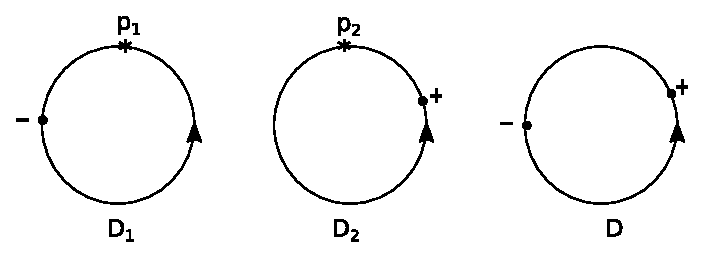
\includegraphics[width=7cm]{connectedsum.eps}
\caption{$D$ is the connected sum of $D_1$ and $D_2$ at points $p_1$ and $p_2$} \label{F: ConnectedSum}
\end{figure}
\end{example}

\begin{theorem}\label{lambda-is-a-subgroup}
The set $\Lambda_G$ is a subgroup of $G$.
\end{theorem}
\begin{proof}
By Theorem \ref{NonEmptyRealizableSet}, $\Lambda_G$ is a non-empty set. Let $\lambda_1, \lambda_2$ be two elements of $\Lambda_G$. Since $\lambda_1, \lambda_2$ are realizable, there exist marked Gauss diagrams $D_1$, $D_2$ and onto homomorphisms $\rho_1: \Pi_{D_1} \to G$, $\rho_2: \Pi_{D_2} \to G$ such that $\rho_1(x_1)=\rho_2(y_1)=\mu$, $\rho_1(v_1)=\rho_2(v_2)=\nu$ and $\rho_1(l_1)=\lambda_1$, $\rho_2(l_2)=\lambda_2$, where $(x_1,l_1)$ and $(y_1,l_2)$ are meridian-longitude pairs of $D_1$ and $D_2$, respectively. Let $D$ be a connected sum of $D_1$ and $D_2$ made over the points lying on arcs $x_1$ and $y_1$. Define a map $\rho: \Pi_D \to G$ such that $\rho(x_i)=\rho_1(x_i)$ $(1 \leq i \leq n)$, $\rho(y_j)=\rho_2(y_j)$ $(1 \leq j \leq m)$ and $\rho(v)=\nu$. It is easy to see that the map $\rho$ is well defined onto homomorphism and $\rho(l)=\lambda_1 \lambda_2$ where $l$ is the longitude corresponding to meridian $x_1$ for $D$. Moreover, let $\bar{D}_1$ be the marked Gauss diagram obtained from $D_1$ by reversing the orientation of circle and sign of chords and nodes. If $\bar{x}_i$ denote the arc in $\bar{D}_1$ which was labeled $x_i$ in $D_1$, then the map $\bar{\rho}_1: \Pi_{\bar{D}_1} \to G$ defined by $\bar{\rho}_1(\bar{x}_i)=\rho_1(x_i)$ is well defined and $\bar{\rho}_1(l)=\lambda_1^{-1}$, where $l$ is the longitude of $\bar{D}_1$ corresponding to the meridian $\bar{x}_1$ for $\bar{D}_1$.
\end{proof}


\medskip

\section{Problems}\label{S: Problems}

In this section we have mentioned some problems.

In \cite{BB-2} are collected different representations of $B_n$. It is possible to construct some extensions of these representations to $VB_n$.

\begin{problem}
Is it true, that any representation of $VB_n$ is equivalent to a virtually symmetric representation?
\end{problem}



\begin{problem}
Under what conditions an irreducible $C_m$-group, $m \geq 2$, can be realized as the group of a marked Gauss diagram?
\end{problem}

\begin{problem} 
Can we give a topological interpretation of equivalence classes of marked Gauss diagrams?
\end{problem}


\newpage
\begin{ack}
Bardakov and Neshchadim are supported by the Russian Science Foundation grant 19-41-02005. Manpreet Singh is supported by IISER Mohali for the PhD Research fellowship. Manpreet Singh also thanks to his supervisor Dr. Mahender Singh for giving him the opportunity to attend VI Russian-Chinese Conference on Knot Theory and Related Topics at NSU (Novosibirsk) and 2nd International Conference on Groups and Quandles in low-dimensional topology at TSU (Tomsk) using his grant, where he had discussions with the first two authors. His visit to Russia was supported by the DST grant INT/RUS/RSF/P-02.
\end{ack}

\begin{thebibliography}{HD}

\bibitem{Bar-1}
V. G. Bardakov, \textit{Virtual and welded links and their invariants}, Sib. Elektron. Mat. Izv., \textbf{2} (2005), 196--199.

\bibitem{BB-1}
V. G. Bardakov, P. Bellingeri, \textit{Groups of virtual and welded links}, J. Knot Theory Ramifications \textbf{23} (2014), no. 3, 1450014, 23 pp.

\bibitem{BB-2}
V. G. Bardakov, P. Bellingeri, \textit{On representations of braids as automorphisms of free groups and corresponding linear representations}, Knot theory and its applications, 285--298, Contemp. Math., \textbf{670}, Amer. Math. Soc., Providence, RI, 2016.

\bibitem{BMN-1}
V. G. Bardakov, Yu. A. Mikhalchishina, M. V. Neshchadim, \textit{Representations of virtual braids by automorphisms and virtual knot groups}, J. Knot Theory Ramifications \textbf{26} (2017), no. 1, 1750003, 17 pp.

\bibitem{BMN-2}
V. G. Bardakov, Yu. A. Mikhalchishina, M. V. Neshchadim, \textit{Virtual link groups}, (Russian) Sibirsk. Mat. Zh. \textbf{58} (2017), no. 5, 989--1003; translation in Sib. Math. J. \textbf{58} (2017), no. 5, 765--777.

\bibitem{BN-2}
V. G. Bardakov, M. V. Neshchadim, \textit{On a representation of virtual braids by automorphisms}, Algebra Logika \textbf{56} (2017), no. 5, 539--547; translation in Algebra Logic \textbf{56} (2017), no. 5, 355--361.

\bibitem{BN-3}
V. G. Bardakov, M. V. Neshchadim, \textit{Knot groups and nilpotent approximability}, (Russian) Tr. Inst. Mat. Mekh. \textbf{23} (2017), no. 4, 43--51; translation in Proc. Steklov Inst. Math. \textbf{304} (2019), suppl. 1, S23--S30.

\bibitem{BK-1}
V. G. Bardakov, A. Kawauchi, \textit{Spatial graph as connected sum of a planar graph and a braid}, arXiv:2006.16072.

\bibitem{BF}
A. Bartholomew, R. Fenn, \textit{Biquandles of small Size and some invariants of virtual and welded knots}, J. Knot Theory Ramifications \textbf{20} (2011), no. 7, 943--954.

\bibitem{BF-1}
A. Bartholomew, R. Fenn, \textit{Update of ``Biquandles of small size and some invariants of virtual and welded wnots"}, arXiv:1004.1320.

\bibitem{BF-2}
A. Bartholomew, R. Fenn, \textit{Quaternionic invariants of virtual knots and links},  J. Knot Theory Ramifications \textbf{17} (2008), no. 2, 231--251.

\bibitem{BH-1}
L. W. Beineke, F. Harary, \textit{Consistency in marked digraphs}, J. Math. Psych. \textbf{18} (1978), no. 3, 260--269.

\bibitem{Bigelow-1}
S. Bigelow, \textit{The Burau representation is not faithful for {$n=5$}}, Geom. Topol. \textbf{3} (1999), 397--404.

\bibitem{BDGGHN-1}
H. U. Boden,  E. Dies, A. I. Gaudreau,  A. Gerlings,  E. Harper,  A. J. Nicas, \textit{Alexander invariants for virtual knots}, J. Knot Theory Ramifications, \textbf{24} (2015), no. 3, 1550009, 62 pp.

\bibitem{BMS-1}
A. M. Brunner, E. J. Mayland, Jr., J. Simon, \textit{Knot groups in $\mathbb{S}^4$ with nontrivial homology}, Pacific J. Math. \textbf{103} (1982), no. 2, 315--324.

\bibitem{CSW-1}
J. S. Carter, D. S. Silver, S. G. Williams, \textit{Invariants of links in thickened surfaces}, Algebr. Geom. Topol. \textbf{14} (2014), no. 3, 1377--1394.

\bibitem{DJK-1}
Q. Deng, X. Jin, L. H. Kauffman, \textit{The generalized Yamada polynomials of virtual spatial graphs}, Topology Appl. \textbf{256} (2019), 136--158.

\bibitem{EL-1}
A. L. Edmonds, C. Livingston, \textit{Symmetric representations of knot groups}, Topology Appl. \textbf{18} (1984), no. 2-3, 281--312.

\bibitem{FM-1}
T. Fleming, B. Mellor, \textit{Virtual spatial graphs}, Kobe J. Math. \textbf{24} (2007), no. 2, 67--85.

\bibitem{FM-2}
T. Fleming, B. Mellor, \textit{Intrinsic linking and knotting in virtual spatial graphs}, Algebr. Geom. Topol. \textbf{7} (2007), 583--601.

\bibitem{Acuna-1}
F. Gonz{\'a}lez-Acu{\~n}a, \textit{Homomorphs of knot groups}, Ann. of Math. (2) \textbf{102} (1975), no. 2, 373--377.

\bibitem{FK-1}
R. Fenn, D. P. Ilyutko, L. H. Kauffman, V. O. Manturov,
\textit{Unsolved problems in virtual knot theory and combinatorial knot theory}, Knots in Poland \RNum{3}. Part \RNum{3}, 9--61, Banach Center Publ., \textbf{103}, Polish Acad. Sci. Inst. Math., Warsaw, 2014.


\bibitem{GH-1}
N. D. Gilbert, J. Howie, \textit{LOG groups and cyclically presented groups}, J. Algebra \textbf{174} (1995), no. 1, 118--131.

\bibitem{Gordon-1}
C. McA. Gordon, \textit{Homology of groups of surfaces in the $4$-sphere}, Math. Proc. Cambridge Philos. Soc. \textbf{89} (1981), no. 1, 113--117.

\bibitem{GPV-1}
M. Goussarov, M. Polyak, O. Viro, \textit{Finite-type invariants of classical and virtual knots}, Topology \textbf{39} (2000), no. 5, 1045--1068.

\bibitem{Hanaki-1}
R. Hanaki, \textit{Pseudo diagrams of knot, links and spatial graphs}, Osaka J. Math. \textbf{47} (2010), no. 3, 863--883.

\bibitem{Johnson-1}
D. Johnson, \textit{Homomorphs of knot groups}, Proc. Amer. Math. Soc. \textbf{78} (1980), no. 1, 135--138.

\bibitem{JL-1}
D. Johnson, C. Livingston, \textit{Peripherally specified homomorphs of knot groups}, Trans. Amer. Math. Soc. \textbf{311} (1989), no. 1, 135--146.

\bibitem{KK-1}
N. Kamada, S. Kamada, \textit{Abstract link diagrams and virtual knots}, J. Knot Theory Ramifications \textbf{9} (2000), no. 1, 93--106.

\bibitem{Kamada-1}
S. Kamada, \textit{Braid presentation of virtual knots and welded knots}, Osaka J. Math. \textbf{44} (2007), no. 2, 441--458.

\bibitem{KT-1}
K. Kanno, K. Taniyama, \textit{Braid presentation of spatial graphs}, Tokyo J. Math. \textbf{33} (2010), no. 2, 509--522.

\bibitem{Kauffman-1}
L. H. Kauffman, \textit{Virtual knot theory}, European J. Combin. \textbf{20} (1999), no. 7, 663--690.

\bibitem{Kauffman-2}
L. H. Kauffman, \textit{Invariants of graphs in three-space}, Trans. Amer. Math. Soc. \textbf{311} (1989), no. 2, 697--710.

\bibitem{KL-1}
L. H. Kauffman, S. Lambropoulou, \textit{Virtual braids and the L-move}, J. Knot Theory Ramifications \textbf{15} (2006), no. 6, 773-811.

\bibitem{KM-1}
L. H. Kauffman, R. Mishra, \textit{Nodal parity invariants of knotted rigid vertex graphs}, J. Knot Theory Ramifications \textbf{22} (2013), no. 4, 1340002, 21 pp.

\bibitem{KKKP-1}
K. Kaur, S. Kamada, A. Kawauchi, M. Prabhakar, \textit{Gauss diagrams, unkotting numbers and trivializing numbers of spatial graphs}, Topology Appl. \textbf{230} (2017), 586--598.


\bibitem{Kim-1}
S. G. Kim, \textit{Virtual knot groups and their peripheral structure}, J. Knot Theory Ramifications \textbf{9} (2000), no. 6, 797--812.

\bibitem{Kulikov-1}
Vik. S. Kulikov, \textit{Alexander polynomials of plane algebraic curves}, Izv. Ross. Akad. Nauk Ser. Mat. \textbf{57} (1993), no. 1, 76--101; translation in Russian Acad. Sci. Izv. Math. \textbf{42} (1994), no. 1, 67--89.

\bibitem{Kulikov-2}
Vik. S. Kulikov, \textit{A geometric realization of $C$-groups}, Izv. Ross. Akad. Nauk Ser. Mat. \textbf{58} (1994), no. 4, 194--203; translation in Russian Acad. Sci. Izv. Math. \textbf{45} (1995), no. 1, 197--206.

\bibitem{Kuperberg-1}
G. Kuperberg, \textit{What is a virtual link$?$}, Algebr. Geom. Topol. \textbf{3} (2003), 587--591.

\bibitem{LLLV-1}
M. Li, F. Lei, F. Li, A. Vesnin, \textit{The Yamada polynomial of spatial graphs obtained by edge replacements}, J. Knot Theory Ramifications \textbf{27} (2018), no. 9, 1842004, 19 pp.

\bibitem{Man}
V. O. Manturov, \textit{On the recognition of virtual braids}, (Russian) Zap. Nauchn. Sem. S.-Peterburg. Otdel. Mat. Inst. Steklov. (POMI)
\textbf{299} (2003), Geom. i Topol. 8, 267--286, 331--332; translation in J. Math. Sci. (N. Y.) \textbf{131} (2005), no. 1, 5409--5419.

\bibitem{Mih}
Yu. A. Mikhalchishina,  \textit{Generalizations of Wada representations and virtual link groups}, (Russian) Sibirsk. Mat. Zh. \textbf{58} (2017), no. 3, 641--659.

\bibitem{Miyazawa-1}
Y. Miyazawa, \textit{The Yamada polynomial for virtual graphs} Intelligence of low dimensional topology 2006, 205--212, Ser. Knots Everything, \textbf{40}, World Sci. Publ., Hackensack, NJ, 2007.

\bibitem{Murakami-1}
J. Murakami, \textit{The Yamada polynomial of spacial graphs and knit algebras}, Comm. Math. Phys. \textbf{155} (1993), no. 3, 511--522.

\bibitem{Neuwirth-1}
L. P. Neuwirth, \textit{Knot groups}, Annals of Mathematics Studies, No. 56, Princeton University Press, Princeton, N. J. 1965 \romannumeral 6 +113 pp.

\bibitem{Petter-1}
O. P. \"Ostlund,  \textit{Invariants of knot diagrams and relations among Reidemeister moves}, J. Knot Theory Ramifications \textbf{10} (2001), no. 8, 1215--1227.

\bibitem{SW}
D. S. Silver, S. G. Williams, \textit{Virtual knot groups}, Knots in Hellas '98 (Delphi), 440--451, Ser. Knots Everything, \textbf{24}, World Sci. Publ., River Edge, NJ, 2000.

\bibitem{SW-1}
D. S. Silver, S. G. Williams, \textit{Alexander groups and virtual links}, J. Knot Theory Ramifications \textbf{10} (2001), no. 1, 151--160.

\bibitem{VV-1}
V. V. Vershinin, \textit{On homology of virtual braids and Burau representation},  J. Knot Theory Ramifications \textbf{10} (2001), no. 5,  795--812.

\bibitem{Wada-1}
M. Wada, \textit{Group invariants of links}, Topology \textbf{31} (1992), no. 2, 399--406.

\bibitem{Yamada-1}
S. Yamada, \textit{An invariant of spatial graphs}, J. Graph Theory \textbf{13} (1989), no. 5, 537--551.

\bibitem{Yetter-1}
D. N. Yetter, \textit{Category theoretic representations of knotted graphs in $\mathbb{S}^3$}, Adv. Math. \textbf{77} (1989), no. 2, 137--155.
\end{thebibliography}
\end{document}

%%%%%%%%%%%%%%%%%%%%%%%%%%%%%%%%%%%%%%%%%%%%%%%%%%%%%
%%%%%%%%%%%%%%%%%%%%%%%%%%%%%%%%%%%%%%%%%%%%%%%%%%%%%
%%%%%%%%%%%%%%%%%%%%%%%%%%%%%%%%%%%%%%%%%%%%%%%%%%%%%
